\documentclass[acmlarge,prologue,table,xcdraw]{acmart}
\newcommand{\rev}[1]{\textcolor[rgb]{0.00,0.00,0.00}{#1}}
\definecolor{outcolor}{rgb}{0.8,0.8,0.8}
\newcommand{\out}[1]{\textcolor{outcolor}{{#1}}}

\AtBeginDocument{%
  \providecommand\BibTeX{{%
    \normalfont B\kern-0.5em{\scshape i\kern-0.25em b}\kern-0.8em\TeX}}}

\setcopyright{acmcopyright}
\copyrightyear{2023}
\acmYear{2023}
\acmDOI{X}


\acmJournal{IMWUT}
\acmVolume{37}
\acmNumber{4}
\acmArticle{111}
\acmMonth{2}




\usepackage{lettrine}

\usepackage{tcolorbox}
\usepackage{listings}
\usepackage{adjustbox}
\usepackage{subcaption}
\usepackage{multirow}
\usepackage{colortbl} 
\usepackage{hhline}
\definecolor{mygray}{gray}{0.8}
\usepackage{pdfpages}



\usepackage{xcolor,color,soul,bm}

\usepackage{tikz}
\usetikzlibrary{backgrounds}



\newcommand{\ds}[1]{\sethlcolor{yellow}\hl{[Dimitris: #1]}}
\newcommand{\mc}[1]{\sethlcolor{lime}\hl{[Marios: #1]}}
\newcommand{\sy}[1]{\sethlcolor{cyan}\hl{[Sofia: #1]}}
\newcommand{\ot}[1]{\sethlcolor{lightgray}\hl{[Other: #1]}}

\newcommand{\todo}[1]{\textcolor{green}{[TODO: #1]}}

\begin{document}

\title{\textit{Beyond Accuracy}: A Critical Review of Fairness in Machine Learning for Mobile and Wearable Computing}


\author{Sofia Yfantidou}
\email{syfantid@csd.auth.gr}
\orcid{0000-0002-5629-3493}
\affiliation{%
  \institution{Aristotle University of Thessaloniki}
  \city{Thessaloniki}
  \country{Greece}
}

\author{Marios Constantinides}
\authornote{Also affiliated with the University of Cambridge, UK.}
\email{marios.constantinides@nokia-bell-labs.coms}
\orcid{0000-0003-1454-0641}
\affiliation{%
  \institution{Nokia Bell Labs}
  \city{Cambridge}
  \country{United Kingdom}
}

\author{Dimitris Spathis}
\authornotemark[1]
\email{dimitrios.spathis@nokia-bell-labs.com}
\orcid{0000-0001-9761-951X}
\affiliation{%
  \institution{Nokia Bell Labs}
  \city{Cambridge}
  \country{United Kingdom}
}



\author{Athena Vakali}
\email{avakali@csd.auth.gr}
\orcid{0000-0002-0666-6984}
\affiliation{%
  \institution{Aristotle University of Thessaloniki}
  \city{Thessaloniki}
  \country{Greece}
}

\author{Daniele Quercia}
\email{daniele.quercia@nokia-bell-labs.com}
\orcid{0000-0001-9461-5804}
\affiliation{%
  \institution{Nokia Bell Labs}
  \city{Cambridge}
  \country{United Kingdom}
}

\author{Fahim Kawsar}
\email{fahim.kawsar@nokia-bell-labs.com}
\orcid{0000-0001-5057-9557}
\affiliation{%
  \institution{Nokia Bell Labs}
  \city{Cambridge}
  \country{United Kingdom}
}


\renewcommand{\shortauthors}{Anonymous, et al.}




\begin{abstract}
The field of \rev{mobile and wearable computing} is undergoing a revolutionary integration of machine learning. Devices can now diagnose diseases, predict heart irregularities, and unlock the full potential of human cognition. However, the underlying algorithms \rev{powering these predictions} are not immune to biases with respect to sensitive attributes (e.g., gender, race), leading to discriminatory outcomes. 
The goal of this work is to explore the extent to which the mobile and wearable computing community has adopted \rev{ways of reporting information about datasets and models to surface and, eventually, counter biases.}
\rev{Our systematic review of papers published in the Proceedings of the ACM Interactive, Mobile, Wearable and Ubiquitous Technologies (IMWUT) journal from 2018-2022 indicates that, while there has been progress made on algorithmic fairness, there is still ample room for growth.} Our findings show that only a small portion (5\%) of published papers adheres to modern fairness reporting, while the overwhelming majority thereof focuses on accuracy or error metrics. \rev{To generalize these results across venues of similar scope, we analyzed recent proceedings of ACM MobiCom, MobiSys, and SenSys, IEEE Pervasive, and IEEE Transactions on Mobile Computing Computing, and found no deviation from our primary result.} In light of these findings, our work provides practical guidelines for the design and development of \rev{mobile and wearable} technologies that not only strive for accuracy but also fairness.


\end{abstract}

\begin{CCSXML}
<ccs2012>
   <concept>
       <concept_id>10003120.10003138</concept_id>
       <concept_desc>Human-centered computing~Ubiquitous and mobile computing</concept_desc>
       <concept_significance>500</concept_significance>
       </concept>
          <concept>
       <concept_id>10010405.10010444.10010446</concept_id>
       <concept_desc>Applied computing~Consumer health</concept_desc>
       <concept_significance>300</concept_significance>
       </concept>
   <concept>
       <concept_id>10010147.10010178</concept_id>
       <concept_desc>Computing methodologies~Artificial intelligence</concept_desc>
       <concept_significance>300</concept_significance>
       </concept>
   <concept>
       <concept_id>10003456.10003457.10003580.10003543</concept_id>
       <concept_desc>Social and professional topics~Codes of ethics</concept_desc>
       <concept_significance>300</concept_significance>
       </concept>
 </ccs2012>
\end{CCSXML}

\ccsdesc[500]{Human-centered computing~Ubiquitous and mobile computing}
\ccsdesc[300]{Applied computing~Consumer health}
\ccsdesc[300]{Computing methodologies~Artificial intelligence}
\ccsdesc[300]{Social and professional topics~Codes of ethics}

\keywords{literature review, survey, machine learning, bias, fairness, responsible artificial intelligence, ubiquitous computing, sensing data}

\received{15 February 2023}

\maketitle

\section{Introduction}\label{section:Introduction}
\glspl{cps} integrate real-time computing and communication capabilities with monitoring and control actions over components in the physical world~\cite{shi_survey_2011}. To face the harshness of the space environment, modern space systems such as satellites and spacecraft require tight coupling between onboard processing, communication (cyber), sensing, and actuation (physical) elements~\cite{klesh_cyber-physical_2012}. The orbit determination and control subsystems on a small spacecraft or in satellites' constellations provide a clear link between onboard processing and sensing elements of the spacecraft's physical environment~\cite{di_mascio_-board_2021}, becoming increasingly critical as small spacecrafts become ever more capable~\cite{klesh_cyber-physical_2012}. In this scenario, digital computing systems representing the decisional part of a \gls{scps} must be designed to be reliable and tolerate faults induced by cosmic radiation. Radiation-induced soft errors such as \glspl{set} and \glspl{seu} can occur more frequently in space than at ground level, creating the need for additional hardware to mitigate detrimental effects on the system~\cite{wachter_survey_2019}.

Various solutions exist to protect electronics from the adverse effects of radiation~\cite{wachter_survey_2019}. Costly radiation-hardened technologies, insulating techniques~\cite{alles_radiation_2011}, and polymer shielding~\cite{shahzad_views_2022} help mitigate soft errors. It is also possible to enhance the fault tolerance capabilities of digital systems by introducing redundancy at different levels in their design flow. Temporal redundancy techniques rely on repeated executions of the same work to determine the correct result~\cite{feng_shoestring_2010}. Spatial or modular redundancy techniques rely on multiple hardware blocks executing the same task and comparing the results~\cite{ginosar_survey_2012}. These approaches rely on rigid schemes for repetition in space and time of redundant blocks or tasks, hence they can severely impact the \gls{ppa} of computing platforms.

The increasing demand for strong processing capabilities in space~\cite{xie_resource-cost-aware_2018} is pushing researchers toward lower-overhead solutions. In recent years, the advent of RISC-V and open-source hardware has encouraged the development of high-performance \glspl{soc} for various domains without licensing or other restrictions. This includes the space domain, where custom modifications to improve properties such as reliability~\cite{di_mascio_open-source_2021} and fault tolerance are often required. Among proposed architectures, heterogeneous systems with multi-core computing clusters have gained traction in the space industry~\cite{ginosar_rc64_2016} due to increased performance and flexibility for computation and \gls{dsp} workloads~\cite{kurth_hero_2018}.
While multiple processors offer increased performance for parallelizable tasks, they also provide a unique opportunity for reliability enhancements: multiple cores can execute identical tasks, comparing their results to detect and react to faults.

In this paper, we introduce a space-ready multi-core RISC-V-based computing system featuring a \gls{hmr} approach. We leverage the independent cores available in a multi-core RISC-V cluster for redundant execution in a dynamically runtime configurable manner and introduce \gls{dcls} and \gls{tcls} modes, extending the On-Demand Redundancy Grouping with \gls{tcls} configurable under reset presented in~\cite{rogenmoser_-demand_2022}.
Our design allows each application to configure its reliability setting according to its requirements, possibly decided at runtime.
% Without sacrificing performance in the general case, this architecture allows for the safe execution of a safety-critical section at a 2.3\% area overhead.
Furthermore, we implement two recovery alternatives, software and hardware-assisted, comparing their impact on the hardware resources and performance in case of a fault. The checking, voting, and switching hardware in the implemented design does not affect the internals of the processor core, allowing for the use of verified RISC-V processor cores without requiring any internal (potentially erroneous) modifications to rapidly build a reliable system.

% The key contributions of this paper are:
% \begin{itemize}
%     \item Combined Dual Core Lockstep and Triple Core Lockstep extensions within a RISC-V-based multi-core cluster.
%     \item Design of a split-lock mechanism to enable runtime-selectable redundant configurations switching in just 550 clock cycles between the available redundant modes. 
%     % \item Exploring the trade-offs for \gls{dmr} and \gls{tmr} on a core-level perspective of the implemented cluster and relating this to classical redundancy mechanisms.
%     \item Design of hardware extensions for fast fault recovery in just 24 clock cycles with only $\sim9\%$ area impact and no timing and performance impacts over the original architecture.
% \end{itemize}
% We propose the first system integrating these functionalities on an open-source RISC-V-based multi-core cluster for fine-tunable reliability vs. performance trade-offs. The key contributions of this paper are:
In summary, we introduce the following key contributions:
\begin{itemize}
    \item A re-configurable computing cluster for Dual-Core Lockstep and Triple-Core Lockstep execution capable of tackling compute-intensive and safety-critical applications. The proposed cluster can be configured so that the computing cores can operate independently if the application requires high-performance capabilities or in Dual/Triple-Core Lockstep mode, depending on the criticality of the executed task.
    \item Robust hardware support for fast fault recovery execution, featuring dedicated Error-Correcting Codes-protected registers to restore the state of the computing cores to the closest reliable state in time. This feature allows the cores to perform cycle-by-cycle backups of their internal state in the protected registers, reducing by $15\times$ the required time to recover from a fault  over the software-based approach.
    \item A runtime-programmable split-lock mechanism allowing for fast switching and re-configuration between the available redundant modes. With these features, it is possible to explicitly define portions of code within a \textit{safety-critical section}, configuring the cores for safe lockstep execution with minimum configuration switching overhead.
\end{itemize}

To validate our proposed approach, we implemented the RISC-V cluster in Global Foundries 22~\si{\nano\meter} technology, achieving up to \SI{430}{\mega\hertz} operating frequency and \SI{1160}{\mega OPS} when configured in independent mode and 617 and 414 MOPS in \gls{dmr} and \gls{tmr} mode, respectively. With only software-based recovery features, the proposed cluster occupies \SI{0.612}{\milli\meter\squared} with just 1.3\% area overhead over the non-redundant configuration, featuring 363 clock cycles time-to-recovery in triple mode. When enhanced with hardware-based recovery features, it provides rapid fault recovery in just 24 clock cycles occupying \SI{0.660}{\milli\meter\squared}, $\sim$9.4\% area overhead over the baseline RISC-V cluster. The proposed split-lock mechanism allows for entering and exiting a redundant mode in just 390 clock cycles for safety-critical code execution.
To foster future research in space-ready computer architecture, we release the proposed architecture as the first fully open-source RISC-V-based multi-core cluster with a finely tunable trade-off between reliability and performance.
\section{Related Work}\label{related-work}
\begin{figure}[tb!]
  \centering
  \includegraphics[width=0.75\linewidth]{figures/teaserCropped.pdf}
  \caption{\textbf{Conceptual differences between ML Fairness and UbiComp datasets.} UbiComp data and models are oftentimes inherently different from those commonly used by the ML fairness community. Figure style inspired by \cite{perez2021wearables}. \label{fig:teaser}}
\end{figure}

Next, we situate our critical review in previous fairness literature covering three broad areas: \emph{a)} far-reaching yet broad surveys; \emph{b)} surveys targeted to specific domains; and \emph{c)} call-for-action works focusing on diverse, representative, and balanced research samples. \\
\smallskip

\noindent\textbf{Broad Fairness Surveys.} Addressing algorithmic bias in ML has been a longstanding issue \cite{caton2020fairness}, despite its recent surge. A number of comprehensive surveys shed light on data and model biases across domains and compared potential mitigation solutions. For example, \citet{caton2020fairness} and \citet{pessach2022review} discussed fairness metrics and categorized mitigation approaches into a widely accepted framework of pre-processing, in-processing, and post-processing methods independently of the application domain. \citet{wan2022processing} focused exclusively on in-processing modeling methods such as adversarial debiasing, disentangled representations, and fairness-aware data augmentation, while  \citet{pessach2022review}'s work provides an overview of emerging research trends, including fair adversarial learning, fair word embeddings, fair recommender systems, and fair visual description. More recently, \citet{mehrabi2021survey} explored data-to-algorithm (e.g., representation bias, measurement bias, aggregation bias, etc.), algorithm-to-user (e.g., popularity bias, user interaction bias, evaluation bias, etc.), and user-to-data (e.g., historical bias, temporal bias, content production bias, etc.) biases, and how these biases are generally encountered in ML practice. Along these lines, \citet{le2022survey} surveyed available datasets for fairness research, including financial, criminological, healthcare, social, and educational datasets. Yet, despite these surveys' considerable contributions, they tend to be of generic nature and rarely discuss data, models, and applications related to an individual community. 
\smallskip

\noindent\textbf{Targeted Fairness Surveys.} Another line of work took a deep dive into well-defined domains (e.g., recommender systems, social networks, healthcare, etc.). A number of works targeted specific ML paradigms, for example, by focusing on fairness for ML for graphs~\cite{choudhary2022survey}, on exploring notions of fairness in clustering~\cite{chhabra2021overview}, and on studying fairness in recommender systems~\cite{li2022fairness}. Another group of works targeted specific unprivileged groups or high-stakes domains. For example, \citet{olteanu2019social} reviewed the literature surrounding social data biases, such as biases in user-generated content, expressed or implicit relations between people, and behavioral traces, while in \cite{sun2019mitigating}, the authors focused specifically on gender bias in Natural Language Processing (NLP). On a different note, \citet{10.1145/3173574.3174156} featured emerging trends for explainable, accountable, and intelligible systems within the CHI community, also discussing notions of fairness. Closer to our work, \citet{mhasawade2021machine} discussed ML fairness in the domain of public and population health, and \citet{xu2022algorithmic} explored algorithmic fairness in computational medicine, which only covers a subset of the broad, interdisciplinary UbiComp research domains.
\smallskip

\noindent\textbf{WEIRD Research.} Last, another strand of fairness work is concerned with what is coined as WEIRD research. WEIRD research refers to a common criticism in the social sciences that much of the research is conducted on a sample of participants that is Western, Educated, Industrialized, Rich, and Democratic (WEIRD). In particular, a comprehensive study conducted by \citet{henrich2010weirdest} in 2010 revealed a significant bias in sample populations. The study found that most research samples come from WEIRD populations, which represent only 12\% of the global population but account for 96\% of research samples. This criticism suggested that using such a narrow and unrepresentative sample of participants can limit the generalizability of the findings to the broader population. Over the past decade, the \textit{CHI} community, which focuses on human-centered design, and the \textit{FAccT} community, which aims to democratize ML and advance the development of responsible artificial intelligence, have become more aware of the potential biases introduced by WEIRD samples. For instance, \citet{linxen2021weird} conducted a meta-study on CHI findings from 2016 to 2020, reporting that 73\% of CHI studies are based on Western populations, representing less than 12\% of the population worldwide, invariably making CHI ``WEIRD'', as it is based on the knowledge and ethics of people who are Western, Educated, Industrialized, Rich, and Democratic. Similarly, a recent meta-study on FAccT proceedings from 2018 to 2021 extracted research topics and identified community values, placing fairness and ML, bias in word embeddings, bias in vision, and racial disparities among the ten largest sub-communities within the conference \cite{laufer2022four}. Yet again, as highlighted in Introduction (Section~\ref{introduction}) in line with prior work \cite{laufer2022four}, ``off-the-shelf'' benchmark datasets are encountered in the majority of published work, while only a $\sim10\%$ of FAccT papers use original, empirical datasets, let alone UbiComp data.

It is evident that research communities other than UbiComp have recently started to explore ways of reporting data and models in a fair manner to surface and, ultimately, address encountered biases. Yet, the state of fairness in the UbiComp community remains unknown, as, at the time of writing, there exists no other survey or position paper in the intersection between UbiComp and fairness. Are our data susceptible to biases? Do our models discriminate against certain demographics, and if so, how do we make them right? These are just a handful of questions we set to provide answers to in this work.


\section{Methodology}
\label{sec:methodology}
Next, we delineate our methodology for conducting this systematic review (\S\ref{conducting} and \S\ref{limitations}) and provide our positionality statement (\S\ref{positionality}).




\begin{figure}[tb!]
  \centering
  \includegraphics[width=\linewidth]{figures/methodologyNew2.pdf}
  \caption{\textbf{Illustration of the literature review methodology.} A high-level overview of the process, including the querying, manual extraction, and filtering, and one of the main results. Note that for readability purposes, we present a simplified version of our query and data extraction. Our query retrieves $\sim55\%$ of all IMWUT publications, while our eligibility assessment filtering ends up with 49 papers ($\sim9\%$ of retrieved papers). We notice that only a very small fraction of all IMWUT papers looks at fairness issues, with only a small deviation across years.  \label{fig:methodology}}
\end{figure}
\subsection{Conducting the Literature Review\label{conducting}}
We followed an established protocol for conducting systematic reviews introduced by \citet{kitchenham2007guidelines} to ensure the quality of included works and limit the initial retrieved papers. At least three authors were involved at each step to minimize the effects of bias and priming. In accordance with this protocol, we initially identified the need for a systematic review, as discussed in Section~\ref{introduction}, namely to explore where UbiComp fairness overlaps with traditional fairness definitions and, more importantly, where it lags behind. Figure~\ref{fig:methodology} provides a high-level overview of the process.
\smallskip 

\noindent\textbf{Paper Identification \& Screening.} 
UbiComp is a relatively new area in Information and Computer Science that crosses several fields, ranging from HCI, Hardware and Software Systems, and Knowledge Discovery and Data Mining. For the scope of this review, we focused on the Proceedings of the ACM on Interactive, Mobile, Wearable and Ubiquitous Technologies (IMWUT), a premier journal in the UbiComp community, also placed among the top-3 publications in HCI.
For the search process, we utilized the ACM Digital Library, focusing on papers that were published in the last five years (between 2018 and 2022) to capture emerging trends in fairness and UbiComp research. We also considered a broader search on Google Scholar but opted not to include it due to scale concerns (e.g.,  the query ``machine learning fairness''  returns approximately 279,000 results on Google Scholar) and the fact that indexed papers may not have undergone peer review. Apart from year filtering, for the most part, we did not limit our search to meta-data, such as titles, keywords, and abstracts, but rather we expanded it to any searchable field, including full text. That excludes the first part of the query, which tries to match terms such as wearable(s) or mobile(s) only in the papers' meta-data, as seen in Figure~\ref{fig:query}. 
\smallskip


\noindent\textbf{Query Definition.} For the definition of our query, we followed similar terminology with relevant review papers in the fairness literature \cite{le2022survey,caton2020fairness}. Additionally, according to Fjeld et al.'s analysis of prominent AI principles documents, \cite{fjeld2020principled}, ``the fairness and non-discrimination theme is the most highly represented theme in our dataset, with every document referencing at least one of its six principles: ``non-discrimination and the prevention of bias'', ``representative and high-quality data'', ``fairness'', ``equality'', ``inclusiveness in impact'', and ``inclusiveness in design'', mostly included in our query's coverage. To capture the industrial perspective, we consulted the Responsible Artificial Intelligence (RAI) white papers issued by large tech companies. Specifically, Google's\footnote{\url{https://ai.google/responsibilities/responsible-ai-practices/?category=fairness}} and Meta's\footnote{\url{https://ai.facebook.com/blog/facebooks-five-pillars-of-responsible-ai/}} RAI principles talk about ``fairness and inclusion'', Amazon's\footnote{\url{https://aws.amazon.com/machine-learning/responsible-machine-learning/}} RAI principles promote ``diversity, equity, and inclusion'' through ``detecting bias''. Similarly, Nokia's\footnote{\url{https://www.bell-labs.com/institute/blog/introducing-nokias-6-pillars-of-responsible-ai/}} RAI fairness pillar talks about ``fairness, non-discrimination, accessibility, and inclusivity'', and Intel's RAI pillars mention ``enabling ethical and equitable AI''. Thus, an iterative refinement process resulted in the query shown in Figure~\ref{fig:query}.

\begin{figure}[tb!]
  \centering
  \includegraphics[width=.75\linewidth]{figures/queryFramed.pdf}
  \caption{\textbf{The query utilized for recovering relevant papers from the ACM Digital Library}. Terms related to UbiComp are highlighted in green, ML in orange, and fairness in purple.\label{fig:query}}
\end{figure}
\smallskip 

\noindent\textbf{Eligibility Assessment.} To further validate our query, we manually inspected all publications from the latest IMWUT proceedings (Volume 6, Issue 4, published in January 2023) ($N=56$) to identify eligible papers for inclusion (see inclusion and exclusion criteria below). In total, we identified seven relevant publications, all of which were also returned by our query. This process was irrelevant to our final paper retrieval (Preferred Reporting Items for Systematic Reviews and Meta-Analyses (PRISMA) \cite{moher2009preferred} flow diagram is pictured in Figure~\ref{fig:prisma}) and served validation purposes only. To ensure the high quality and relevance of the included papers, we defined appropriate exclusion criteria that helped us determine the included papers:
\begin{enumerate}
    \item Papers that do not provide a quantitative assessment of at least one empirical or artifact contribution in ubiquitous computing (UBI);
    \item Papers that do not include a quantitative assessment of bias or performance discrepancy in their evaluation with regard to sensitive attributes, such as age, gender, race, disability, religion, and sexual orientation, among others (FAIR);
    \item Papers that discuss different domains, such as natural language processing or computer vision without incorporating a UbiComp component (DOM);
    \item Papers that refer to bias in a different context, such as the bias-variance trade-off or the bias parameter in neural networks (CON). 
\end{enumerate}

\begin{figure}[tb!]
  \centering
  \includegraphics[width=.95\linewidth]{figures/prismaNew2.pdf}
  \caption{\textbf{PRISMA flow diagram for paper inclusion}. Out of the 611 papers retrieved by our query after the screening, only 9\% ($N=49$) did not check any exclusion criterion and thus were included in the literature review.  The majority of the retrieved papers were false positives, highlighting the importance of the eligibility assessment.  \label{fig:prisma}}
\end{figure}
\noindent\textbf{Inclusion \& PRISMA Statement.} Finally, the sequential execution of the steps above, as depicted in Figure~\ref{fig:prisma}, led to our review's included papers. Overall, we screened 523 papers after date filtering and duplicate elimination. After carefully screening these papers, we excluded 474 based on our exclusion criteria. In detail, 31 papers did not provide any quantitative assessment of a UbiComp contribution (UBI: 6.5\%), 394 papers did not provide any fairness assessment (FAIR: 83.1\%), 2 papers did not discuss a UbiComp component (DOM: <0.5\%), 42 papers referred to bias in a different context (CON: 8.9\%), and finally, 5 papers were excluded for other reasons (OTHER: 1.1\%). Hence, we included 49 papers in our review\footnote{To foster reproducibility, upon acceptance, we intend to release the review data and codebooks}. 


\subsection{Methodological Limitations}
\label{limitations}
While we have made every effort to ensure broad coverage of papers relevant to fairness in UbiComp studies, our search for literature might not be comprehensive and exhaustive. However, covering IMWUT as a prominent academic venue for ubiquitous computing research allowed us to capture emerging trends. Besides, we intended to provide insights and research directions to the IMWUT community; therefore, we narrowed down our research to IMWUT proceedings as opposed to the broader community by including the proceedings of, for example, PerCom, SenSys, MobiSys, or medical journals such as JMIR. We also acknowledge that despite our best efforts to pick literature-driven keywords and manually validate the retrieved results, the output might well have produced both false positives and false negative results. 



\subsection{Positionality Statement\label{positionality}}
Understanding researcher positionality is essential to demystifying our lens on data collection and analysis~\cite{frluckaj2022gender, havens2020situated}. We situate this review paper in a Western country (REDACTED FOR REVIEW) in the 21\textsuperscript{st} century, writing as authors who primarily work as academic and industry researchers. We identify as two females and four males, and our shared backgrounds include HCI, ML, and ubiquitous computing. 

\section{Results\label{sec:results}}

In the discussion of our results, we looked into bias in both models and data in the included papers. \textit{Model bias} refers to systematic errors that are introduced into ML algorithms due to the underlying assumptions in the data, algorithms, or the learning process itself, leading to unfair or unequal outcomes for certain sensitive groups. In the following sections, we explore the state of fairness in the UbiComp community (Section~\ref{mf1}), the ethical risks and opportunities in the domain and how they can inspire the choice of fairness metrics (\S\ref{mf2}), and ultimately, we capture alternative notions of fairness that the UbiComp community has perhaps indirectly adopted (and adapted) to capture the particularities of the domain (\S\ref{mf3}). \textit{Data bias} refers to errors occurring because certain user groups, or generally elements, within a dataset are more heavily weighted and/or represented than others. A biased dataset does not accurately represent a model’s target domain, causing skewed outcomes, low performance, and systematic errors. In the sections below, we also discuss reported or historical biases relevant to the domain's data modalities (\S\ref{historical-biases}) and explore diversity in UbiComp datasets and research teams (\S\ref{weird}).


\setlength\arrayrulewidth{2pt}\arrayrulecolor{gray}
\begin{table}[]
\caption{A summary of the included papers categorized by application domain, fairness enhancement mechanism, sensitive attribute, and bias metrics. High-stakes health application papers are the most active in the UbiComp community regarding fairness. While all included papers talk about fairness with respect to one or more sensitive attributes, the vast majority do not offer enhancement mechanisms.}
\label{tab:summary}
\resizebox{\textwidth}{!}{%
\begin{tabular}{p{2.2in}p{1.55in}p{1.7in}p{2in}p{1in}}
\rowcolor[HTML]{1C9E77} 
{\color[HTML]{FFFFFF} \textbf{APPLICATION DOMAIN}} &
  {\color[HTML]{FFFFFF} \textbf{FAIRNESS MECHANISM}} &
  {\color[HTML]{FFFFFF} \textbf{SENSITIVE ATTRIBUTE}} &
  {\color[HTML]{FFFFFF} \textbf{FAIRNESS METRICS}} &
  {\color[HTML]{FFFFFF} \textbf{PAPERS}} \\
\rowcolor[HTML]{F3F3F3} 
Health (26.5\%) &
  Preprocessing &
  Gender &
  \cellcolor[HTML]{F3F3F3} &
  \cite{10.1145/3351281} \\
\rowcolor[HTML]{F3F3F3} 
 &
   &
  Age &
  \multirow{-2}{*}{\cellcolor[HTML]{F3F3F3}Accuracy} &
   \\
\rowcolor[HTML]{F3F3F3} 
 &
   &
  Health Condition &
  MAE &
  \cite{10.1145/3328927} \\ \cline{2-2}
\rowcolor[HTML]{F3F3F3} 
 &
  In-processing &
  Socioeconomic Status &
  Precision, Sensitivity, Specificity &
  \cite{10.1145/3411835} \\ \cline{2-2}
\rowcolor[HTML]{F3F3F3} 
 &
  None &
  Gender &
  Accuracy, AUC-ROC, F1, Sensitivity, Specificity, MAPE, Error rate &
  \cite{10.1145/3478127,10.1145/3534583,10.1145/3478107,10.1145/3534595,10.1145/3463503} \\
\rowcolor[HTML]{F3F3F3} 
 &
   &
  Age &
  Accuract, AUC-ROC, Sensitivity, Specificity, Pearson's r, Error rate &
  \cite{10.1145/3478127,10.1145/3381016,10.1145/3534583,10.1145/3478098,10.1145/3463503} \\
\rowcolor[HTML]{F3F3F3} 
 &
   &
  Health Condition &
  Accuracy, AUC-PRC, AUC-ROC, F1, Precision, Sensitivity, Specificity, RMSE &
  \cite{10.1145/3328917,10.1145/3534578,10.1145/3478107,10.1145/3463503} \\
\rowcolor[HTML]{F3F3F3} 
 &
   &
  Physiology &
  F1, Sensitivity, Specificity &
  \cite{10.1145/3478107} \\
\rowcolor[HTML]{F3F3F3} 
 &
   &
  Race &
  AUC-ROC, MAE &
  \cite{10.1145/3534583,10.1145/3517225} \\
\rowcolor[HTML]{FFFFFF} 
Privacy \& Security (12.2\%) &
  None &
  Age &
  Error rate &
  \cite{10.1145/3448113} \\
\rowcolor[HTML]{FFFFFF} 
 &
   &
  Health Condition &
  Precision, P-value &
  \cite{10.1145/3264899,10.1145/3494960} \\
\rowcolor[HTML]{FFFFFF} 
 &
   &
  Physiology &
  Accuracy &
  \cite{10.1145/3161198,10.1145/3264944,10.1145/3351273} \\
\rowcolor[HTML]{FFFFFF} 
 &
   &
  Religion &
   &
  \cite{10.1145/3161198} \\
\rowcolor[HTML]{F3F3F3} 
Human-Activity Recognition (10.2\%) &
  Pre-processing &
  Gender &
  F1 &
  \cite{10.1145/3517252} \\
\rowcolor[HTML]{F3F3F3} 
 &
   &
  Age &
   &
   \\
\rowcolor[HTML]{F3F3F3} 
 &
   &
  Physiology &
   &
   \\ \cline{2-2}
\rowcolor[HTML]{F3F3F3} 
 &
  In-processing &
  Gender &
  F1 &
  \cite{10.1145/3397330} \\ \cline{2-2}
\rowcolor[HTML]{F3F3F3} 
 &
  \cellcolor[HTML]{F3F3F3} &
  Gender &
  Accuracy &
  \cite{10.1145/3397311} \\
\rowcolor[HTML]{F3F3F3} 
 &
  \cellcolor[HTML]{F3F3F3} &
  Physiology &
  F1 &
  \cite{10.1145/3397313} \\
\rowcolor[HTML]{F3F3F3} 
 &
  \multirow{-3}{*}{\cellcolor[HTML]{F3F3F3}None} &
  Miscellaneous &
  MSE &
  \cite{10.1145/3161201} \\
\rowcolor[HTML]{FFFFFF} 
Behavioral Sensing \& Emotion (10.2\%) &
  Pre-processing &
  Gender &
  Accuracy &
  \cite{10.1145/3351246} \\
\rowcolor[HTML]{FFFFFF} 
 &
   &
  Age &
  Accuracy, MAE &
  \cite{10.1145/3517249,10.1145/3351246,10.1145/3369820} \\
\rowcolor[HTML]{FFFFFF} 
 &
   &
  Nationality &
  Accuracy &
  \cite{10.1145/3351246} \\ \cline{2-2}
\rowcolor[HTML]{FFFFFF} 
 &
  None &
  Gender &
  Accuracy, Coefficient of determination &
  \cite{10.1145/3448089,10.1145/3478126} \\
\rowcolor[HTML]{F3F3F3} 
Sound, Voice \& Hearing (10.2\%) &
  Pre-processing &
  Gender &
  Accuracy &
  \cite{10.1145/3494969} \\ \cline{2-2}
\rowcolor[HTML]{F3F3F3} 
 &
  None &
  Gender &
  Error rate, Mel cepstral distortion &
  \cite{10.1145/3161601,10.1145/3550338,10.1145/3550293} \\
\rowcolor[HTML]{F3F3F3} 
 &
   &
  Age &
  Error rate &
  \cite{10.1145/3550293} \\
\rowcolor[HTML]{F3F3F3} 
 &
   &
  Physiology &
  Accuracy, MAE &
  \cite{10.1145/3517253} \\
\rowcolor[HTML]{F3F3F3} 
 &
   &
  Nationality &
  Error rate &
  \cite{10.1145/3161601} \\
\rowcolor[HTML]{FFFFFF} 
Motion, Gaze, Gesture \& Touch (8.2\%) &
  None &
  Gender &
  Accuracy &
  \cite{10.1145/3432235,10.1145/3351255} \\
\rowcolor[HTML]{FFFFFF} 
 &
   &
  Age &
   &
   \\
\rowcolor[HTML]{FFFFFF} 
 &
   &
  Health Condition &
  Error rate &
  \cite{10.1145/3494999} \\
\rowcolor[HTML]{FFFFFF} 
 &
   &
  Physiology &
  Accuracy &
  \cite{10.1145/3191772,10.1145/3432235} \\
\rowcolor[HTML]{F3F3F3} 
Mobility \& Navigation (8.2\%) &
  Pre-processing &
  Gender &
  Accuracy &
  \cite{10.1145/3191774} \\
\rowcolor[HTML]{F3F3F3} 
 &
   &
  Age &
   &
   \\
\rowcolor[HTML]{F3F3F3} 
 &
   &
  Physiology &
   &
   \\ \cline{2-2}
\rowcolor[HTML]{F3F3F3} 
 &
  In-processing &
  Gender &
  Accuracy, AUC-ROC, F1 &
  \cite{10.1145/3494990} \\
\rowcolor[HTML]{F3F3F3} 
 &
   &
  Age &
   &
   \\
\rowcolor[HTML]{F3F3F3} 
 &
   &
  Socioeconomic Status &
   &
   \\ \cline{2-2}
\rowcolor[HTML]{F3F3F3} 
 &
  None &
  Gender &
  F1 &
  \cite{10.1145/3314407} \\
\rowcolor[HTML]{F3F3F3} 
 &
   &
  Age &
  F1 &
   \\
\rowcolor[HTML]{F3F3F3} 
 &
   &
  Miscellaneous &
  Accuracy &
  \cite{10.1145/3411807} \\
\rowcolor[HTML]{FFFFFF} 
Miscellaneous (8.2\%) &
  Pre-processing &
  Miscellaneous &
  Accuracy &
  \cite{10.1145/3534585} \\ \cline{2-2}
\rowcolor[HTML]{FFFFFF} 
 &
  None &
  Gender &
  Required rate of return &
  \cite{10.1145/3432193} \\
\rowcolor[HTML]{FFFFFF} 
 &
   &
  Age &
  Required rate of return &
   \\
\rowcolor[HTML]{FFFFFF} 
 &
   &
  Marital Status &
  Required rate of return &
   \\
\rowcolor[HTML]{FFFFFF} 
 &
   &
  Physiology &
  P-value &
  \cite{10.1145/3550312} \\
\rowcolor[HTML]{FFFFFF} 
 &
   &
  Language &
  Error rate &
  \cite{10.1145/3161187} \\
\rowcolor[HTML]{F3F3F3} 
Cognition \& Attention (6.1\%) &
  None &
  Age &
  RMSE &
  \cite{10.1145/3411811} \\
\rowcolor[HTML]{F3F3F3} 
 &
   &
  Physiology &
  MSE &
  \cite{10.1145/3161164} \\
\rowcolor[HTML]{F3F3F3} 
 &
   &
  Miscellaneous &
  Accuracy, AUC-ROC, Precision, Sensitivity, MAE, MSE, Pearson's r &
  \cite{10.1145/3432235,10.1145/3448111}
\end{tabular}%
}
\end{table}

\subsection{What is the State of Fairness in UbiComp?\label{mf1}}
Before delving into details about fairness assessment, enhancement mechanisms, and metrics documented in the included papers, we summarize the approaches adopted by the UbiComp community in Table~\ref{tab:summary}. 
The table presents all included papers, categorized per application domain, sensitive attributes, and fairness mechanisms and metrics. In summary, out of the 523 retrieved papers, a small portion of 9\% ($N_{included}=49$) were included in the review, which in turn make up only 5\% of all IMWUT publications between 2018 and 2022, highlighting the timeliness and necessity of this work. \\


\tikzstyle{background rectangle}=[thin,draw=black]
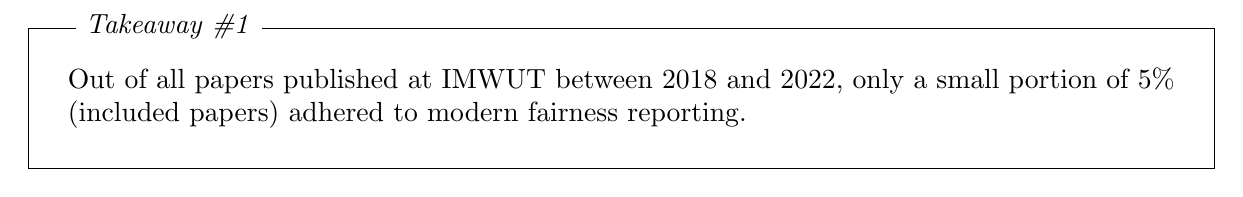
\begin{tikzpicture}[show background rectangle]
\node[align=justify, text width=40em, inner sep=1em]{
Out of all papers published at IMWUT between 2018 and 2022, only a small portion of 5\% (included papers) adhered to modern fairness reporting. 
};
\node[xshift=3ex, yshift=-0.7ex, overlay, fill=white, draw=white, above 
right] at (current bounding box.north west) {
\textit{Takeaway \#1}
};
\end{tikzpicture} 
\smallskip

To identify appropriate application domains, we consulted the past four years (2019-2022) of UbiComp tracks and sessions to identify commonalities in discussed themes. We grouped together tracks' themes between years based on their similarity and relevance to the included papers. This process led us to the identification of ten domains: \textit{Health}; \textit{Human-Activity Recognition}; \textit{Behavioral Sensing \& Emotion}; \textit{Cognition \& Attention}; \textit{Motion, Gaze, Gesture \& Touch}; \textit{Sound, Voice \& Hearing}; \textit{Mobility \& Navigation}; \textit{Privacy \& Security}; \textit{Localization}, and \textit{Miscellaneous}. We encountered all but one theme (localization) in the included papers, which is not unreasonable given localization's usually low-stakes applications and, thus, less relevance to fairness. Health was the most commonly encountered domain, accounting for more than one in four papers, while Cognition \& Attention was the least common, accounting for only $\sim6\%$ of included papers. 

\begin{figure*}[t!]
    \centering
    \begin{subfigure}[t]{0.45\textwidth}
        \centering
        \includegraphics[width=.95\linewidth]{figures/cloudAllCropped.pdf}
    \end{subfigure}%
    \hspace{1em}%
    \begin{subfigure}[t]{0.45\textwidth}
        \centering
        \includegraphics[width=.95\linewidth]{figures/cloudIncludedCropped.pdf}
    \end{subfigure}
    \caption{\textbf{Keyword differences of retrieved (left) and included (right) papers}. Frequent keywords in both retrieved and included papers are colored in dark grey. Over-represented keywords in the retrieved papers are colored in green, while over-represented keywords in the included papers are colored in pink. Even within UbiComp, the privacy, audio, and vision communities are trailblazers in ML fairness. \label{fig:wordclouds}}
\end{figure*}
Figure~\ref{fig:wordclouds} provides an overview of the discussed domains, as captured by the papers' keywords. It also serves as a validation to the domains' categorization, as many categories (e.g., \textit{Health}; \textit{Human-Activity Recognition}; \textit{Motion, Gaze, Gesture \& Touch}; \textit{Sound, Voice \& Hearing} and \textit{Privacy \& Security}) also appear in the keyword clouds. Deep learning,  ML, and human activity recognition are among the most frequently overlapping keywords (colored in dark grey). Over-represented keywords in the retrieved papers (colored in green) include mobile sensing, wearables, Internet of Things (IoT), Radio-frequency identification (RFID), and self-supervised learning. Over-represented keywords in the included papers (colored in pink) include mobile health, Post-traumatic stress disorder (PTSD), acoustic sensing, computer vision, privacy, and gesture recognition. 

\subsubsection{Fairness Enhancement Mechanisms} 
For each application domain, we categorized its papers based on three fairness enhancement mechanisms \cite{pessach2022review,caton2020fairness}: a) \textit{pre-processing}; b) \textit{in-processing}; and c) \textit{post-processing} mechanisms. It is often infeasible to eliminate all sources of unfairness and guarantee fairness. Yet, the goal is to surface and mitigate biases as much as possible through fairness enhancement mechanisms.
\smallskip

\noindent \textbf{Pre-processing mechanisms} involve altering the training data before feeding it into a ML algorithm. Within UbiComp, preliminary but effective mechanisms include fair data representation. For instance, during data collection, \citet{10.1145/3328927} equally included both healthy subjects and subjects with Chronic Obstructive Pulmonary Disease (COPD) in their dataset for respiratory rate monitoring using smartwatches, leading to non-significant differences in model performance across health condition. Similarly, \citet{10.1145/3534585} employed a fairness-aware client selection mechanism for federated learning to ensure equal representation for subjects with worse connectivity.\footnote{While Internet connectivity is not a sensitive attribute per se, it has been linked with socioeconomic status, race, nationality, gender, and age, all of which are sensitive attributes \cite{united2021almost}.} 
Post data collection, \citet{10.1145/3494969} performed data balancing, conditioned on the sensitive attribute, managing to narrow the impact of gender voice differences on their speech recognition model. Similarly, a strand of work explored data splitting, conditioned on the sensitive attribute (gender, age, BMI, skin tone, country, and health condition) to enable model personalization \cite{10.1145/3369820,10.1145/3351246,10.1145/3517249,10.1145/3494969,10.1145/3351281}. More advanced mechanisms suggest modifying feature representations so that a subsequent classifier will be fairer. For example, \citet{10.1145/3191774} improved the performance of their activity detection model by normalizing the window-level features across gender and physiology, yet their model remained dependent on sensitive attributes. Similarly, in line with prior work~\cite{locatello2019fairness}, \citet{10.1145/3517252} utilized disentangled representations, aiming to isolate relevant activity patterns from redundant noises such as gender, age, and physiological differences, reducing the effect of such covariate factors. However, they did not manage to completely separate the activity signals from the redundancy, attributing it to the diversity limitations of Human-Activity Recognition datasets.
\smallskip

\noindent \textbf{In-processing mechanisms} involve modifying the ML algorithms to account for fairness during training. In the included papers, \citet{10.1145/3411835} altered their logistic regression model for Post-traumatic stress disorder (PTSD) screening to include sensitive attributes in its parameters, having observed statistically significant inter-group and intra-group differences based on gender and socioeconomic status. Their alteration led to a statistically significant improvement in performance across groups. On a similar note, \citet{10.1145/3397330} devised a multi-task loss function consisting of activity, subject, and gender loss. However, they noticed unbalanced performance, with the performance on gender attribute learning being around 11\% lower than the performance on the other two tasks. Finally, in quantifying the causal effect of individual mobility on health status, \citet{10.1145/3494990} considered certain sensitive attributes, such as age and socioeconomic status, as confounding variables in their causal model, after establishing that such attributes can affect the correlation between mobility and health.
However, they noted that due to dataset privacy constraints in reporting demographic variables, potential unobserved confounding variables, such as occupation, employment, and education, might have been missed, highlighting the conflict between fairness and privacy \cite{chang2021privacy}.
\smallskip

\noindent \textbf{Post-processing mechanisms} involve altering the output scores of the ML model to make decisions fairer. However, due to the relatively late stage in the learning process in which they are applied, post-processing mechanisms commonly obtain inferior results \cite{woodworth2017learning}. They are also considered too invasive or discriminatory since they deliberately damage accuracy for some subjects to compensate others \cite{pessach2022review}; hence they are less frequently preferred in practice. Perhaps not surprisingly, such mechanisms are not present in the included papers.

Despite the notable efforts of the aforementioned pioneering works in the UbiComp community, 3 out of 4 included papers did not report any fairness enhancement mechanism, regardless of the presence of bias in their models. This is partly due to a lack of consideration for fairness-related harms, but it is also connected with the nature of several UbiComp works: artifact contributions, proof of concept, and early-stage technology development, where performance is prioritized. \\




\tikzstyle{background rectangle}=[thin,draw=black]
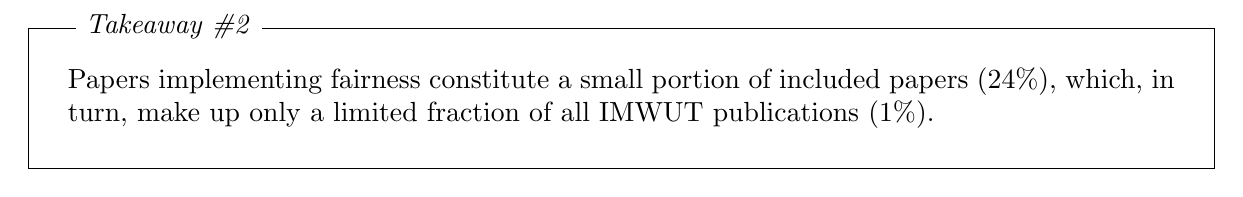
\begin{tikzpicture}[show background rectangle]
\node[align=justify, text width=40em, inner sep=1em]{
Papers implementing fairness constitute a small portion of included papers (24\%), which, in turn, make up only a limited fraction of all IMWUT publications (1\%). 
};
\node[xshift=3ex, yshift=-0.7ex, overlay, fill=white, draw=white, above 
right] at (current bounding box.north west) {
\textit{Takeaway \#2}
};
\end{tikzpicture} 



\begin{figure*}[t!]
    \centering
    \begin{subfigure}[t]{0.65\textwidth}
        \centering
        \includegraphics[width=\linewidth]{figures/deploymentCropped.pdf}
        \caption{\textbf{Frequency of in-the-lab versus in-the-wild deployments along with fairness assessment results.} \label{fig:deployment}}
    \end{subfigure}%
    \hspace{1em}%
    \begin{subfigure}[t]{0.3\textwidth}
        \centering
        \includegraphics[width=\linewidth]{figures/biasCropped.pdf}
        \caption{\textbf{Sensitive attributes along with reported fairness results.}\label{fig:bias}}
    \end{subfigure}
    \caption{\textbf{Bias results across deployment settings and sensitive attributes}. The figures visualize the fairness assessment results reported in the included papers against deployment setting (left) and sensitive attributes (right). ``B'' indicates a bias towards one or more sensitive attribute(s), while ``U'' indicates an unbiased model. In \ref{fig:deployment} (left), the deployment environment distribution is relatively balanced, but the reported fairness assessments differ with in-the-wild studies reporting significantly less unbiased results. In \ref{fig:bias}, gender, age, and physiology are amongst the most frequently assessed attributes, while, surprisingly, race and language are understudied. Note that a single paper might assess more than one sensitive attribute; hence the sum may exceed the number of included papers ($N=49$).\label{fig:alternative}}
\end{figure*}

\subsubsection{Sensitive Attributes \& Biases\label{sensitive-attributes-biases}} 
The categorization of sensitive attributes is inspired by the EU Charter of Fundamental Rights that prohibits any discrimination based on any ground such as sex, age, race, ethnic or social origin, genetic features, language, and religion or belief, among others \cite{eu2012charter}. In line with such declarations and prior fairness work \cite{pessach2022review}, UbiComp works investigate a variety of sensitive attributes individually or combined: \textit{gender}, \textit{age}, \textit{physiology} (e.g., height, weight), \textit{health}, \textit{language}, \textit{nationality}, \textit{socioeconomic status}, \textit{religion}, \textit{race}, \textit{occupation}, and \textit{marital status}, as seen in Table~\ref{tab:summary}. 


Nevertheless, some attributes are better represented than others in the included papers, with gender and age being at the top (mentioned in almost 9 out of 10 included papers), followed by physiology and health condition (mentioned in 4 out of 10 included papers), as seen in Figure~\ref{fig:bias}.  Surprisingly, attributes with long-history of discrimination in ML, such as race, language, and nationality \cite{compas,manzini2019black,lee2018detecting}, are rarely encountered in the UbiComp literature, with only two papers discussing racial discrepancies in model performance. Yet, UbiComp is far from immune to such discrepancies. \citet{sjoding2020racial} uncovered racial and ethnic biases in pulse oximetry, while \citet{hutiri2022bias} reported language biases in speech recognition.

In line with such findings, our review of UbiComp's work highlighted biases in ML models across all sensitive attributes and a wide range of UbiComp applications. Gender biases have been reported in monitoring sleep posture with wireless signals \cite{10.1145/3397311}, opioid usage tracking \cite{10.1145/3478107}, diaphragmatic breathing monitor based on acoustic signals \cite{10.1145/3534595}, and speech recognition via accelerometer sensors \cite{10.1145/3494969}. Age biases have been reported in medication adherence monitoring through gait assessment \cite{10.1145/3351281}, fatigue estimation via smartphone tapping frequency \cite{10.1145/3478098}, mobility purpose and route choice inference \cite{10.1145/3314407}, and neural activation prediction \cite{10.1145/3534583}. Biases based on physiological measurements have been reported by \citet{10.1145/3517253} in fine-grained activity sensing (e.g., eye blinking, finger tracking) using acoustic signals against people of small stature, by \citet{10.1145/3550293} in vital sign monitoring through acoustic sensing against obese or overweight people, and by \citet{10.1145/3161198} in image processing with binocular thermal cameras against people of non-average height. Similarly, a model for early detection and burden estimation of AFib under-performed for long-term AFib patients compared to their healthy counterparts \cite{10.1145/3463503}, while a wearable-based clinical opioid use tracker showed bias against chronic opioid users \cite{10.1145/3478107}. Regarding less explored sensitive attributes, \citet{10.1145/3161198} encountered model biases in user authentication via binocular thermal cameras for hijab wearers, a proxy for religion, while \citet{10.1145/3161187} uncovered language biases in speech and keyboard text entry for non-English speakers. It is worth noting that all included papers explore notions of group fairness rather than individual and subgroup fairness (detailed in 
\S\ref{sec:background}). \\


\tikzstyle{background rectangle}=[thin,draw=black]
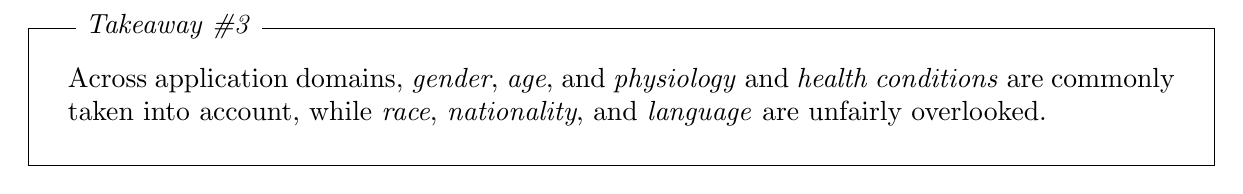
\begin{tikzpicture}[show background rectangle]
\node[align=justify, text width=40em, inner sep=1em]{
Across application domains, \emph{gender}, \emph{age},  and \emph{physiology} and \emph{health conditions} are commonly taken into account, while \emph{race}, \emph{nationality}, and \emph{language} are unfairly overlooked.



};
\node[xshift=3ex, yshift=-0.7ex, overlay, fill=white, draw=white, above 
right] at (current bounding box.north west) {
\textit{Takeaway \#3}
};
\end{tikzpicture} 

\subsubsection{Fairness Metrics} 
Metrics for performance evaluation monopolize UbiComp fairness assessment and reporting as shown in Table~\ref{tab:summary}. Classification metrics, such as Accuracy, Area under the ROC Curve (AUC-ROC), and F1-Score, etc., and regression metrics, such as Root-mean-square Error (RMSE), Mean Absolute Error (MAE), and Mean Absolute Percentage Error (MAPE) highlight the interest of the UbiComp community for such tasks. There exist two challenges, though, with UbiComp's take on fairness: Firstly, how does one define a threshold in performance evaluation above which a model is considered unfair across sensitive attributes? For instance, if an AFib detection model has 85\% accuracy on healthy adults and 80\% accuracy on the elderly, should it be considered fair or unfair? This challenge holds for the entirety of ML fairness research, as there are seldom clear-cut answers. Secondly, how does one perform fairness assessment in regression or multi-class classification scenarios, both wildly understudied areas in the fairness domain compared to binary classification \cite{mohamed2022normalise}? This challenge especially holds for UbiComp. To see how, consider that 1 out of 2 included papers did not discuss binary classification.

To answer the first question, one could employ a statistical hypothesis test, such as the Student's t-test, for comparing samples' performance across sensitive attributes, a practice also adopted by a portion of the included papers. Yet the choice of a statistical test is far from straightforward, each incorporating strict assumptions. For example, a key assumption of the paired Student's t-test is that the observations in each sample are independent, which is not the case in k-fold cross-validation, a common practice in ML model evaluation, leading to an incorrect calculation of the t-statistic and a misleading interpretation of the results and p-value \cite{dietterich1998approximate}. Better alternatives proposed include McNemar's Test or $5\times2$ cross-validation and its refinements \cite{dietterich1998approximate,nadeau1999inference}. Note that more than 1 in 4 included papers (27.7\%) did not use any statistical significance testing in their assessment. 
Another limitation of performance-based assessment of fairness is the assumption that performance optimization and fairness criteria always overlap. For instance, an AFib detection algorithm might be optimized for accuracy \cite{bumgarner2018smartwatch}, but in fairness assessment, one might also want to ensure equal false negative and false positive rates across groups. An alternative to statistical significance testing on performance metrics, also adopted by the FAccT community, is the usage of fairness metrics; namely several measures, such as demographic parity or equalized odds, that enable the detection of bias in one's data or model, as briefly discussed in Section~\ref{sec:background}. Once a fairness metric is obtained, it is common practice to apply the ``4/5 rule'' or ``80\% rule'', which states that ``the selection rate of any group should be not less than 4/5 than the one of the group with the highest selection rate'' \cite{castelnovo2022clarification}. This refers to the guidelines established by the US Equal Employment Opportunity Commission (EEOC) \cite{usguidelines}, which are frequently cited as one of the few legal frameworks that rely on a specific definition of fairness, particularly the concept of demographic parity. Yet, there is no single fairness definition, metric, or ``fair'' threshold that will universally apply to different applications. The rule should only be used as a ``rule of thumb'' and is dependent on the application domain. For example, in high-stakes applications (e.g., health), would we consider ``acceptable'', or fair, a model for arterial oxygen saturation estimation with 80\% accuracy on Asian, Black, and Hispanic patients and 95\% accuracy on White patients---even though it abides by the ``4/5 rule''? It is worth noting that we did not identify any fairness metrics in the included papers, indicating the disjointedness between the UbiComp and the FAccT communities.  

Regarding the second question, nearly half of the included papers (47\%) engage in regression or multi-class classification tasks, such as respiratory rate detection and human-activity recognition, respectively. Yet, the most common ML paradigm explored in fairness research is binary classification \cite{mohamed2022normalise}, with most fairness metrics and enhancement mechanisms specifically targeted to such tasks. In one of the few works about fair regression, \citet{agarwal2019fair} introduced two definitions of fairness in regression: \textit{statistical parity}, which asks that the prediction be statistically independent of the sensitive attribute, and
    \textit{bounded group loss}, which asks that the prediction error restricted to any sensitive group remain below some predefined threshold. A popular way to quantify fairness in regression is to compare the outcome distribution across sensitive attributes using the Kullback–Leibler divergence \cite{joyce2011kullback}, or Kolmogorov-Smirnov test for goodness of fit \cite{massey1951kolmogorov}. If the test fails to reject the null hypothesis that the distributions come from the same population, it is considered fair. Otherwise, it is determined that there is at least one sensitive group whose distribution does not come from the same population. However, this does not reveal which distributions are different (i.e., which group the model is biased against), and what are the characteristics of such differences (e.g., differences in mean, variance, skewness), requiring a subsequent analysis \cite{agarwal2019fair}. Similarly, popular ML fairness libraries, such as AIF360\footnote{\url{https://aif360.mybluemix.net/}} and FairLearn\footnote{\url{https://fairlearn.org/}}, at the time of writing, do not include any regression-specific fairness metrics' implementations. In multi-class classification scenarios, computing ``standard'' fairness metrics such as equalized odds and demographic parity can be challenging due to the lack of a clear definition of ``positive'' and ``negative'' classes. To address this issue, one feasible solution is to transform the problem into multiple binary classification problems and then aggregate the results. More recent approaches include the Combined Error Variance (CEV) and Symmetric Distance Error (SDE) metrics \cite{blakeney2021simon,blakeney2021measure} to quantitatively evaluate the class-wise bias of multi-class classification models. \\


\tikzstyle{background rectangle}=[thin,draw=black]
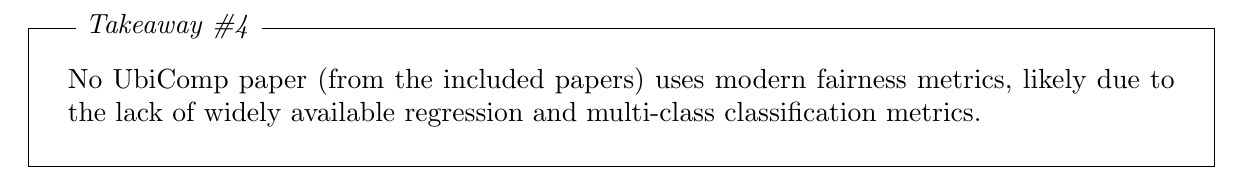
\begin{tikzpicture}[show background rectangle]
\node[align=justify, text width=40em, inner sep=1em]{
No UbiComp paper (from the included papers) uses modern fairness metrics, likely due to the lack of widely available regression and multi-class classification metrics.
};
\node[xshift=3ex, yshift=-0.7ex, overlay, fill=white, draw=white, above 
right] at (current bounding box.north west) {
\textit{Takeaway \#4}
};
\end{tikzpicture} 

\subsection{Model Consequences: Ethical Risks versus Opportunities\label{mf2}}
It is no longer a matter of debate that ML has and will have a major impact on UbiComp, and by extension, on society; human authentication \cite{10.1145/3351273}, early detection and burden estimation of AFib \cite{10.1145/3463503}, respiratory rate monitoring \cite{10.1145/3463503}, and opioid use tracking \cite{10.1145/3478107} are only a handful of examples that reinforce this argument. The discussion has now shifted to determining the extent and specifics of this impact. In other words, it is given that ubiquitous ML will have an impact on society; what is now being questioned is the specifics of who will feel the effects, how, where, and when they will be felt.

To concretize these questions, the Scientific Committee of the AI4People\footnote{An Atomium–European Institute for Science, Media and Democracy initiative.} has categorized the chief ethical opportunities offered by artificial intelligence in ``four fundamental points in the understanding of human dignity and flourishing'' \cite{floridi2018ai4people}: ``who we want to become'' (enabling self-realization), ``what we can do'' (enhancing human agency), ``what we can achieve'' (increasing individual and societal capabilities), and ``how can we interact with each other and the world'' (cultivate societal cohesion). Ethical opportunities within UbiComp span across all four points: UbiComp-based automation of mundane tasks, such as gait-based human authentication \cite{10.1145/3351273}, speech transcription \cite{10.1145/3161187}, or gesture recognition \cite{10.1145/3432235} may easily mean more time spent more intelligently (self-realization). UbiComp-based augmentation of human intelligence, such as cognitive load measurement \cite{10.1145/3448111}, or cognitive performance prediction \cite{10.1145/3448111} may enable humans to do more, better, and faster (human agency). UbiComp-based innovations in medicine, such as PTSD screening \cite{10.1145/3411835},  medication adherence monitoring \cite{10.1145/3351281}, or post-operative complications prediction \cite{10.1145/3534578}, may reinvent society by radically enhancing what humans are collectively capable of (individual and societal capabilities), while UbiComp-supported cooperative work, such as social context inference \cite{10.1145/3478126}, may support societal cohesion and collaboration (societal cohesion).

However, we must also consider the ethical risks associated with inadvertent overuse and deliberate or unintended misuse of UbiComp technologies, stemming, for example, from lack of awareness, conflicting interests, greed, or malicious intent. Simply put, ethical risks are the most likely and predictable negative consequence of any action or inaction. And while performance optimization is frequently fueled by the potential of ethical opportunities, fairness assessment is also driven by ethical risks. Oftentimes, fairness considerations in ML systems are influenced by the question: What is the consequence of the predictive outcome? The answer to this question can drive the choice of suitable fairness definitions and metrics but is far from straightforward. For instance, in the case of AFib detection, a false negative outcome might prove deadly. Yet, ``\textit{deploying a system with a high false alarm rate can add anxiety to people}'' \cite{10.1145/3463503}. Similarly, in predicting postoperative complications in pancreatic cancer patients, a false negative outcome can deprive a patient of much-needed care. However, ``\textit{many false positive errors, \emph{[...]} means the patients without complications are incorrectly predicted to be at high risk. As a result, clinicians may decide to provide pre-habilitation to reduce their risk of surgical complications or even cancel the surgery. However, pre-habilitation delays surgery and the patients might miss their opportunity for successful recovery and surgery is the only cure for the cancer.}'' \cite{10.1145/3534578}. On the contrary, in speech-based human identification scenarios, false positive outcomes are critical in preventing unauthorized access, as ``\textit{existing voiceprint-based authentication often suffers from various voice spoofing attacks}'' \cite{10.1145/3448113}. 

Prioritizing predictive outcomes becomes even more challenging once perceived through their sociotechnical context. Oftentimes UbiComp technologies are built and evaluated as if they were fully autonomous, while in reality, they operate in a complicated sociotechnical system moderated by institutional structures and human stakeholders (the ``framing trap'' \cite{selbst2019fairness}). For instance, in opioid use tracking \cite{10.1145/3478107}, and drug-seeking behavior sensing \cite{10.1145/3328917} applications ---both encountered in the included papers--- the consequence of a predictive outcome depends on the assumption of punitive or restorative justice \cite{hadzi2019restorative}. According to traditional punitive justice, punishment serves as a deterrent for wrongdoing, and a means to alter behavior. However, restorative justice takes a different approach, recognizing that punishment alone does not repair the harm caused to the community and relationships. Additionally, restorative believes that relying solely on punishment can result in individuals becoming dependent on external factors rather than internal self-control to modify their behavior \cite{van2014restoring}. As an example, if a ubiquitous substance abuse detection technology is adopted by a restorative system, a false negative outcome might derive an individual struggling with drug addiction from crucial access to rehabilitation services. For instance, ``\textit{if such a device were found to be reliable, it could be used to monitor early treatment response and therefore could allow clinicians to more rapidly optimize patient care}'' \cite{10.1145/3328917}. On the contrary, if the exact same technology is employed as part of a punitive system, then a false negative outcome might lead to a wrongful accusation or conviction. 

Nevertheless, fear, ignorance, and misplaced concerns should not inhibit the UbiComp community from innovation and realizing ethical opportunities for individual and societal good. On the contrary, mindful use of ML is conscious of our commonalities and differences across sensitive groups, as well as the factors within and outside the community's control, and serves as a framework to act with a sense of responsibility and fostering trust. \\
 


\tikzstyle{background rectangle}=[thin,draw=black]
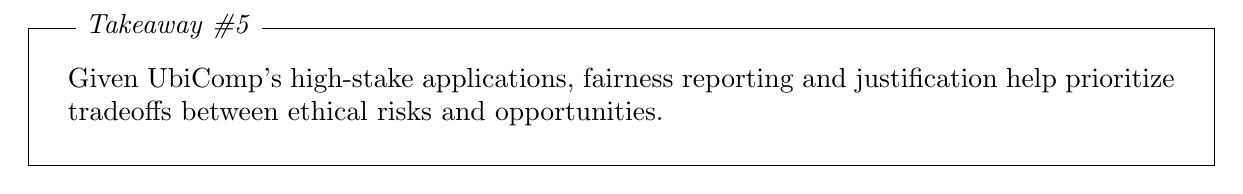
\begin{tikzpicture}[show background rectangle]
\node[align=justify, text width=40em, inner sep=1em]{
Given UbiComp's high-stake applications, fairness reporting and justification help prioritize tradeoffs between ethical risks and opportunities. 








};
\node[xshift=3ex, yshift=-0.7ex, overlay, fill=white, draw=white, above 
right] at (current bounding box.north west) {
\textit{Takeaway \#5}
};
\end{tikzpicture} 



\subsection{How does UbiComp Capture Alternative Notions of Fairness?\label{mf3}}
Previously, we have established that only a small fraction of IMWUT works (5\%) follow conventional fairness definitions, where fairness is defined with respect to one or more sensitive attributes. Yet, we believe such definitions do not do full justice to the community's work, which strives for ``fairer'' models, perhaps not across sensitive attributes, but across differing experimental conditions. In particular, we noticed that, in evaluating new UbiComp systems, artifacts, or applications, the community aims for generalizable and robust models by performing ablations studies, comparing deployment settings, and personalizing models for users and groups. As an indication, in the retrieved papers, almost one out of two papers (44\%) reported an ablation study or a deployment setting comparison in their results, while in the included papers, 57\% did so. 
\smallskip 


\noindent\textbf{Ablation Studies.} In an ablation study, one or more components of the model are systematically removed or modified, and the performance of the model is evaluated after each change. By comparing the performance of the original model with the performance of the modified models, researchers can determine the importance of each component and gain insights into the functioning of the model across diverse conditions, ensuring its generalizability and robustness. In the included papers, ablation studies take the form of performance evaluation comparisons based on: \textit{user-related components}, \textit{device-related components}, \textit{environmental components}, \textit{experimental components}, and \textit{domain-specific components}. In particular \textit{user-related components} include user motion and orientation during data collection in sleep posture monitoring~\cite{10.1145/3397311}, breathing monitoring~\cite{10.1145/3534595}, gesture recognition~\cite{10.1145/3432235}, user identification~\cite{10.1145/3264944}, and heart activity monitoring~\cite{10.1145/3478127}, as well as aesthetics, such as hair or clothing in fine-grained activity sensing~\cite{10.1145/3517253}, breathing and vital sign monitoring~\cite{10.1145/3534595,10.1145/3550293}, and user identification~\cite{10.1145/3161198,10.1145/3351273}. \textit{Device-related components} include device type, sampling rate, and operating system, as well as device placement and orientation in activity and gaze tracking~\cite{10.1145/3517253,10.1145/3494999}, vital sign monitoring and physiological sensing~\cite{10.1145/3550293,10.1145/3517225}, speech recognition via built-in sensors and speech synthesis \cite{10.1145/3494969,10.1145/3550338}, and user behavior sensing \cite{10.1145/3448089}. \textit{Environmental components} include ambient noise, light, and temperature that might affect data quality of acoustic~\cite{10.1145/3517253,10.1145/3448113,10.1145/3550293} or video~\cite{10.1145/3191772,10.1145/3161164,10.1145/3517225,10.1145/3161198} signals, respectively, or random passers-by that might affect model performance on the individual for human identification \cite{10.1145/3351273}. Regarding experimental setup, few included papers studied the effect of equipment placement (i.e., distance, angle) and characteristics (i.e., range) on the model's robustness in activity sensing~\cite{10.1145/3517253} and vital sign monitoring using acoustic signals~\cite{10.1145/3534595,10.1145/3550293}. Apart from such common components, the choice of components to consider in an ablation study is highly domain-dependent. \textit{Domain-specific components} have no limitations and can range from screen size in scrolling interaction experiments \cite{10.1145/3351255} to food structure in food-related artifact development \cite{10.1145/3550312}.
\smallskip 

\noindent\textbf{Deployment Setting.} Beyond ablation studies, a study's deployment setting, ranging from in-the-lab to in-the-wild, can significantly impact its outcomes. While laboratory settings can provide controlled environments for experimentation, they may not accurately reflect the complexities of the real world in which the applications are deployed. As a result, in-the-wild (or in-situ) studies have emerged as an alternative approach, focusing on evaluating the situated design experience of UbiComp. Such studies provide insight into how new ubiquitous technologies are adopted in real-world settings \cite{rogers2007s}. Figure~\ref{fig:deployment} shows the distribution of in-the-lab and in-the-wild studies in the included papers, along with their reported fairness assessment results. We see that perhaps not surprisingly, in-the-lab studies prevail ($\sim55\%$), which can be explained by the nature of numerous IMWUT papers presenting cutting-edge artifacts or early-stage model development work. Nevertheless, $\sim38\%$ of included papers conduct in-the-wild studies, and a small fraction of papers ($\sim7\%$) compare and report results for both deployment settings. An interesting point to be made here is that while 4 out of 10 in-the-lab studies do not identify biases in their models, this number falls to 0.5 in 10 for in-the-wild studies. This confirms our intuition that controlled environments might conceal biases that would emerge once a model is deployed in the real world.
\smallskip 

\noindent\textbf{Personalization.} In 20\% of the papers included, personalization was reported as a commonly used approach for gaining insights on performance differences between individuals. In particular, several works trained separate personalized models for inference on a single subject \cite{10.1145/3351281,10.1145/3264944,10.1145/3161601} or a group of subjects sharing a common characteristic. For instance, \citet{10.1145/3369820} built personalized models for different age groups ``\textit{illustrating differences in communication patterns across age demographics that can impact model performance}''. Similarly, \citet{10.1145/3517249} utilized age-specific models for predicting the right moment for providing mobile safety help, as ``\textit{different ages in the sample have a significant influence on supportable moment predictions}''. \citet{10.1145/3517225} developed personalized models based on skin tone for camera-based, non-contact photoplethysmography, as ``\textit{previous work had already highlighted [skin tone and gender] issues with the Plane-Orthogonal-to-Skin [method]}''. \citet{10.1145/3494969} developed gender-specific models for speech recognition, as ``\textit{women’s voice is generally thinner and higher in pitch}'', while \citet{10.1145/3397313} explored BMI-based models for detecting eating activities via a multi-sensor necklace, due to ``\textit{differences in movement patterns while eating, change in the distance of the proximity sensor from the neck, and difference in posture during the eating activity}''. \\



\tikzstyle{background rectangle}=[thin,draw=black]
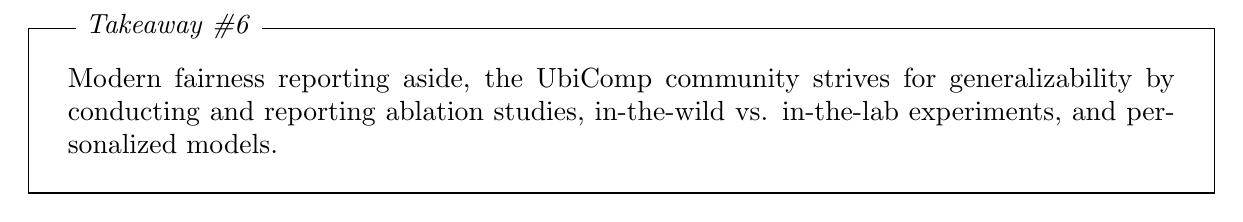
\begin{tikzpicture}[show background rectangle]
\node[align=justify, text width=40em, inner sep=1em]{
Modern fairness reporting aside, the UbiComp community strives for generalizability by conducting and reporting ablation studies, in-the-wild vs. in-the-lab experiments, and personalized models.
};
\node[xshift=3ex, yshift=-0.7ex, overlay, fill=white, draw=white, above 
right] at (current bounding box.north west) {
\textit{Takeaway \#6}
};
\end{tikzpicture} 
\smallskip









\subsection{Is UbiComp Susceptible to Data Biases?\label{historical-biases}}
UbiComp is inherently multimodal; even the relatively small subset of included papers contained heterogeneous modalities of input data such as audio, video, images, text, and sensor data (e.g., accelerometer, gyroscope, temperature, electrodermal activity (EDA) sensors). These different modalities may be related or complementary and can provide a more complete and nuanced representation of a given phenomenon than any one data modality alone.
\smallskip


\noindent \textbf{Biases in audio} (used by 18\% of included papers) are well-reported in fairness research communities \cite{hutiri2022bias,markl2022language,10.1145/3485730.3493448}. UbiComp posed no exception, with such biases surfacing from the included papers. Several works discovered biases in acoustic signals dependent on body size, a potential proxy for gender, physiology, and race. Specifically, \citet{10.1145/3517253}  generically reported ``\textit{higher respiration [detection] error [...] due to [...] weaker chest motions and smaller body size}'', while \citet{10.1145/3534595} specifically reported bias against women due to ``\textit{different physiological structures}'', which led to ``\textit{the reflective surface of women [being] smaller than that of men, which encodes less information}''. Similarly, \citet{10.1145/3550293} found that acoustic signals for heartbeat monitoring were biased against people with larger BMI, as ``larger BMI [would] make the thoracic muscle thicker and block the weak heartbeat signals''. 
\smallskip

\noindent \textbf{Biases in video and image} (used by 20\% of included papers) are also well-studied in fairness literature \cite{dasari2021evaluation, nowara2020meta}. 
Within UbiComp, \citet{10.1145/3534583} attributed performance discrepancies in computer vision models to data-related factors regarding participants’ identity, gender, age, race, ethnicity, and Fitzpatrick skin type~\cite{fitzpatrick1988validity}. In line with this discourse, \citet{10.1145/3161198} identified video biases related to physiology, such as height, and appearance features such as hair or head covering, potentially proxies for gender and religion, respectively. Specifically, they encountered certain issues during video capture: ``\textit{As [the tallest participants] moved closer to the cameras, both participant's heads moved above the viewing range of the [...] camera}''; or ``\textit{[the algorithm] often measured the participant at their forehead rather than the top of their head [...] due to [the participant's] long, thick, curly hair}''; and finally, `` \textit{when [the participant] turned away from the camera and only her hijab was visible [the algorithm] was unable to detect her presence as different from the background}''.

Some of these biases are easier to distinguish as demographic information is integrated into the data. For example, gender, age, physiology, and race may be inferred from video, while gender, language, and possibly age and race may be inferred from speech signals. However, sensor signals ---the most prevalent data modality used by the UbiComp community--- are more challenging and equally susceptible to data biases. Prior research has reported racial and ethnic biases in pulse oximeters \cite{sjoding2020racial}. Additionally, gender biases may be a concern for electrocardiogram (ECG) quality, given that certain ECG metrics, such as the PR interval, heart rate, QRS duration, and lead voltages, exhibit gender-based differences \cite{xue2014can}. Even the most inconspicuous sensors, such as heart rate and acceleration sensors, are shown to be correlated with health, fitness, and demographic characteristics \cite {spathis2021self}.
\smallskip

\noindent \textbf{Biases in sensor signals} (used by 51\% of included papers) also surfaced during our review. These biases could be attributed either to measurement inaccuracy or concept drift phenomena in signal patterns (i.e., distributions of data change over time, making machine learning models less accurate without updates \cite{lu2018learning}). For example, \citet{10.1145/3351281} reported decreased accuracy in gait detection via accelerometer and gyroscope measurements for elderly users as ``Human gait patterns inevitably change with the increase of age. The so-called aging effect may affect the detection accuracy of [the] system''. Furthermore, \citet{10.1145/3494969} encountered inaccuracies in accelerometer-based speech recognition, ``Since women's voice is generally thinner and higher in pitch, [and] it may be harder for [the] accelerometer to preserve voice feature''. Similarly, in speech synthesis from accelerometer measurement, \citet{10.1145/3550338} also found gender-based differences in the accelerometer's ability to preserve the voice feature. In particular, ``\textit{[...] the frequency bands of male speakers are lower than those of female speakers. The lower pitch of the male speaker makes it practicable to encompass vocal traits with a lower sampling frequency with fewer losses on the high-frequency bands}''. On a different note, \citet{10.1145/3397313} utilized multiple sensors (i.e., inertial measurement unit (IMU), proximity, and ambient light sensors) for eating activity detection. They detected performance discrepancies for participants with large BMI, attributing them to data-related factors, such as ``\textit{[...] differences in movement patterns while eating, change in the distance of the proximity sensor from the neck, and difference in posture during the eating activity}''. It is crucial to understand that such biases are not straightforward to distinguish. On the contrary, they remain hidden, blended into time-series signals, or, even worse, propagated to inferred high-level signals such as steps, physical activity, and sleep. Such challenges call for additional care and demographic meta-data for post hoc fairness analysis.\\


\tikzstyle{background rectangle}=[thin,draw=black]
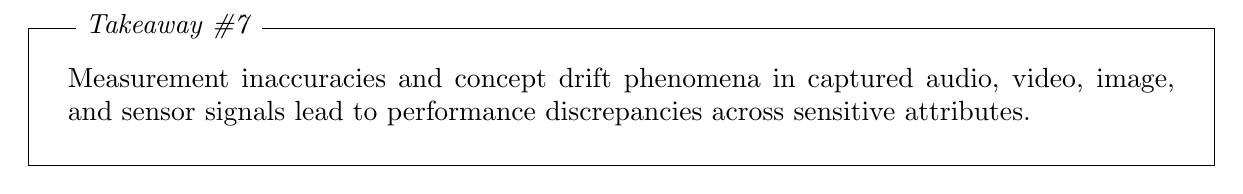
\begin{tikzpicture}[show background rectangle]
\node[align=justify, text width=40em, inner sep=1em]{
Measurement inaccuracies and concept drift phenomena in captured audio, video, image, and sensor signals lead to performance discrepancies across sensitive attributes.
};
\node[xshift=3ex, yshift=-0.7ex, overlay, fill=white, draw=white, above 
right] at (current bounding box.north west) {
\textit{Takeaway \#7}
};
\end{tikzpicture} 
\smallskip


\begin{figure}[tb!]
  \centering
  \includegraphics[width=\linewidth]{figures/weirdNew.pdf}
  \caption{\textbf{Analysis of sensitive attributes and data size}. The bar plots show the percentage of papers reporting certain sensitive attributes (left) and the (mean) sample size in the subset of papers reporting that attribute (right). Note that for age and country, we report the mean sample age and the number of papers originating from the USA, respectively. Sample demographics reporting is not standardized and frequently incomplete, with race, employment status, and education being the least reported sensitive attributes ($\leq20\%$). While UbiComp samples tend to be gender-balanced, they are still WEIRD, as they consist of predominantly White, highly-educated, and US-based subjects.\label{fig:weird}}
\end{figure}

\subsection{How WEIRD is UbiComp?\label{weird}}
Inspired by previous call-to-action papers appearing in other communities about diversity in datasets and sample demographics \cite{linxen2021weird,schlesinger2017intersectional}, we performed an analysis of UbiComp datasets with regard to sensitive attribute distributions. We chose the WEIRD acronym coined by \citet{henrich2010weirdest} as a starting point to inspect how Western, Educated, Industrialized, Rich, or Democratic UbiComp really is. 

Figure~\ref{weird} presents the results of our analysis. The bar plot on the left (a) shows the percentage of papers reporting certain sensitive attributes: gender, age, race, education, employment, and sample country. The bar plot on the right (b) gives the mean sample size within each subset of papers reporting that sensitive attribute. Note that the mean was used, despite its sensitivity to outliers, because the median tends to be less accurate and more biased than the mean when sample sizes are small. In particular, gender was the most reported sensitive attribute in IMWUT datasets. 86\% of included papers ($N=42$) disclosed this information. Within these 42 papers, the mean sample size was 136 users, and the mean number of females in the sample was 71. Evidently, the community has made a step in the right direction by engaging in a conscious effort to achieve more balanced, diverse, and representative datasets. Yet, there is plenty of room for improvement. The second most-reported attribute was only reported in 4 out of 10 papers ($N=20$), and the mean sample age within these papers was 31 years old. For comparison, the maximum mean age reported was 66 years. In a world that is rapidly aging \cite{world2015world}, the UbiComp community is predominantly developing and testing on young populations. Such a finding is in line with prior work, reporting that within the fall detection domain, for example, datasets usually comprise imitated falls performed by younger people while they are intended for deployment on older people \cite{sucerquia2017sisfall}. Finally, only 12\% of included papers ($N=6$) mentioned the participants' race. Within this subset, the mean sample size was 112 users, 88 of which were White (79\%). Even though these numbers should be taken with a grain of salt, due to the small number of papers, it is worth pointing out that not only race is a wildly overlooked sensitive attribute (see results in Section~\ref{sensitive-attributes-biases}), but non-White populations are significantly underrepresented within UbiComp datasets. There is a risk that models underperform for non-White users, but this fact may go unnoticed as there is no effort to check for it. For instance, \citet{10.1145/3463503} could not assess the impact of skin tone on AFib detection ``due to the unbalanced dataset where the majority (88.7\%) of participants were White''.

Confirming IMWUT's WEIRDness, out of the 42 papers for which the participants' country (a proxy for Western) is reported or can be inferred, 36 (86\%) engaged with US samples. 
China (26\%) and Switzerland (7\%) completed the top-3 of country representation. Note that the percentages do not sum up to 100 because of papers with more than one sample country. Concerning education (a proxy for Educated), 20\% of included papers ($N=10$) reported relevant information, with a median sample size of 144 users, 92 of which were college-educated (80\%). This is perhaps not surprising, as in the early stages of development in UbiComp, participant recruitment frequently takes place within the universities and from the researchers' close circle. Regarding employment status (a proxy for Industrialized and Rich), it was only reported in 14\% of included papers ($N=7$), with a mean sample size of 208 users, of which 152 were employed.

Digging deeper into IMWUT's WEIRDness, we found that out of the 49 included papers, 32 (65\%) included at least one author with a US-based affiliation. To evaluate whether the participants' countries are more diverse than the authors' locations, we analyzed the author affiliations reported in the 42 articles that also contained information about the participants' countries. Out of those, only 3 papers (7\%) recruited at least part of their sample from a country different than the authors' location. In the remaining cases, participants were from the same country as at least one of the affiliated institutions. These results demonstrate that the vast majority of IMWUT authors (93\%) recruit samples within the country they are located. This proportion is in line ---even though larger--- with similar analyses in other communities, such as CHI \cite{linxen2021weird}. This is possibly due to the requirements of in-the-lab or artifact-based research common within the UbiComp community.\\


\tikzstyle{background rectangle}=[thin,draw=black]
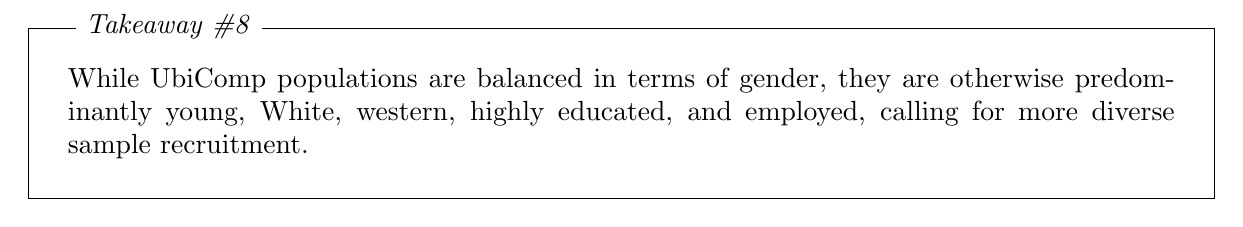
\begin{tikzpicture}[show background rectangle]
\node[align=justify, text width=40em, inner sep=1em]{
While UbiComp populations are balanced in terms of gender, they are otherwise predominantly young, White, western, highly educated, and employed, calling for more diverse sample recruitment.
};
\node[xshift=3ex, yshift=-0.7ex, overlay, fill=white, draw=white, above 
right] at (current bounding box.north west) {
\textit{Takeaway \#8}
};
\end{tikzpicture} 



 

\section{\rev{How is fairness discussed across UbiComp venues?}}\label{generalizability}

\begin{table}[]
\caption{\textbf{To generalize these results across venues of similar scope, we analyzed recent proceedings of ACM MobiCom, MobiSys, and SenSys, and IEEE Trans. of Mobile Computing and Pervasive Computing, and found no deviation from our primary result.} Out of the 514 total papers published in 2022 in these venues, 245 were retrieved by our query, and only 12 complied with our screening eligibility criteria.}
\label{tab:venues}
\begin{tabular}{llll}
\rowcolor[HTML]{1C9E78} 
{\color[HTML]{FFFFFF} \textbf{Venue}} & {\color[HTML]{FFFFFF} \textbf{\#Published (2022)}} & {\color[HTML]{FFFFFF} \textbf{\#Retrieved (\% total)}} & {\color[HTML]{FFFFFF} \textbf{\#Included (\% total)}} \\
{ACM IMWUT}           & {154}                          & {131 (85\%)}                       & {15 (10\%)}                        \\
\rowcolor[HTML]{F3F3F3} 
MobiCom                               & 56                                                 & 25 (45\%)                                              & 0 (0\%)                                               \\
MobiSys                               & 38                                                 & 18 (47\%)                                              & 3 (8\%)                                               \\
\rowcolor[HTML]{F3F3F3} 
SenSys                                & 52                                                 & 8 (15\%)                                               & 2 (4\%)                                               \\
IEEE Pervasive                        & 49                                                 & 15 (31\%)                                              & 2 (4\%)                                               \\
\rowcolor[HTML]{F3F3F3} 
IEEE Trans. Mob. Comp.              & 319                                                & 179 (56\%)                                             & 5 (2\%)                                               \\
{\textbf{Total}}           & {\textit{668}}                & {\textit{376 (56\%)}}             & {\textit{27 (4\%)}}                                  
\end{tabular}
\end{table}
\rev{To evaluate how our results generalize across UbiComp venues, we reviewed last year's (2022) publications from relevant mobile and wearable computing conferences and journals. Specifically, we reviewed ACM SIGMOBILE-sponsored events, including the International Conference on Mobile Computing and Networking (MobiCom, $N_{2022}=56$), the International Conference on Mobile Systems, Applications, and Services (MobiSys, $N_{2022}=38$), and the ACM Conference on Embedded Networked Sensor Systems (SenSys, $N_{2022}=52$), and relevant IEEE journals, including IEEE Pervasive Computing (IEEE Pervasive, $N_{2022}=49$) and IEEE Transactions on Mobile Computing (IEEE Trans. Mob. Comp., $N_{2022}=319$). Following the methodology described in Section~\ref{sec:methodology}, out of 245 retrieved papers, 12 papers complied with our screening and eligibility criteria: none from MobiCom (0\% inclusion rate), 3 from MobiSys (8\%), 2 from SenSys (4\%), 2 from IEEE Pervasive (4\%), and 5 from IEEE Trans. Mob. Comp. (2\%). Table~\ref{tab:venues} summarizes our analysis. The papers came from domains overlapping with those identified at IMWUT: \textit{Sound, Voice, \& Hearing} (33.3\%) \cite{chatterjee2022clearbuds,jin2022earhealth,xie2021hearsmoking,xu2020leveraging}, \textit{Privacy \& Security} (25\%) \cite{wu2022g2auth,zhao2020fingertip,li2020characterising}, \textit{Health} (25\%) \cite{xu2022hearing,stasak2022breaking,lamichhane2022econet}, \textit{Motion, Gaze, Gesture \& Touch} (8.3\%) \cite{cao2022gaze}, and \textit{Mobility \& Navigation} (8.3\%) \cite{hu2020mathsf}.}

\rev{Of all reviewed papers, we found that only 2\% adhered to fairness reporting ($N_{included}=12$), slightly below half the percentage published in IMWUT, highlighting the timeliness and the need for this review (takeaway \#1). At the same time, none introduced fairness enhancement mechanisms or utilized fairness metrics (takeaways \#2 and \#4). Similarly to IMWUT, physiology \cite{chatterjee2022clearbuds,xu2022hearing,xie2021hearsmoking,xu2020leveraging,zhao2020fingertip}, age \cite{jin2022earhealth,wu2022g2auth,stasak2022breaking}, gender \cite{jin2022earhealth,wu2022g2auth}, and health conditions \cite{stasak2022breaking,lamichhane2022econet} were the most frequently considered protected attributes, whereas there were no mentions of race, nationality, or language (takeaway \#3). Nevertheless, once again, in-the-wild deployments and ablation studies were widespread amongst reviewed papers, considering user-related \cite{jin2022earhealth,cao2022gaze,xie2021hearsmoking,xu2020leveraging}, device-related \cite{wu2022g2auth,cao2022gaze,li2020characterising}, environmental \cite{chatterjee2022clearbuds,wu2022g2auth,xie2021hearsmoking,xu2020leveraging,zhao2020fingertip}, experimental \cite{xu2022hearing,cao2022gaze,xie2021hearsmoking,zhao2020fingertip}, and domain-specific components \cite{zhao2020fingertip} (takeaway \#6). Finally, following our IMWUT findings, users were recruited mainly from the USA (57\%) and China (43\%). They were generally balanced in terms of gender with a median of 10 females but predominantly young ($\mu_{age}=23.1)$. However, due to the lack of standardization in demographics reporting, data were insufficient to draw conclusions about race, education, and employment distributions (takeaway \#8).} 

\rev{Overall, while we acknowledge the limitations of considering a single publication for this review, these findings provided an indication of the generalizability of our results across UbiComp venues.} 
\section{Discussion}
\label{sec:discussion}
By screening 523 papers published at IMWUT between 2018 and 2022, we found that only a small portion \rev{(5\%)} adhered to fairness reporting, while \rev{most} focused on accuracy or error metrics. By delving into the smaller number of 49 papers, we surfaced biases in machine learning data and models across several sensitive attributes and application domains that would otherwise remain scattered in the UbiComp literature. Yet, the identified lack of diverse datasets in IMWUT publications could result in biases remaining undetected in the absence of heterogeneous demographics. To quantify such biases, included papers primarily employed performance evaluation instead of fairness metrics, while challenges in fairness assessment were found in regression and multi-class classification scenarios. \rev{We also validated the generalizability of our findings across UbiComp venues by reviewing retrieved publications from the past year.}
Similar to other communities, defining fairness in UbiComp was not a simple task and involved considering its sociotechnical context, its ethical risks, and opportunities. Nevertheless, in an effort to employ fairness in practice ---sensitive attributes aside--- we found that the community has been striving for generalizability through ablation studies, real-world deployments, and personalization.

\begin{figure}[]
  \centering
  \includegraphics[page=1,trim={0 0 0 0.2in},width=0.65\linewidth]{figures/guidelinesBlack.pdf}
  \includegraphics[page=2,width=0.65\linewidth]{figures/guidelinesBlack.pdf}
    \includegraphics[page=3,trim={0 1.1in 0 0},width=0.65\linewidth]{figures/guidelinesBlack.pdf}
  \caption{\textbf{Recommendations for ``Fairness by design'' in UbiComp.} \rev{Guidelines for researchers for performing fairness assessments accompanied by implementation details and examples. Fairness should not be an afterthought but starts with problem definition and data collection.}\label{fig:recommendations}} 
\end{figure}

Drawing from these findings and borrowing from the ``Privacy by design'' literature \cite{fjeld2020principled,cavoukian2009privacy}, we propose a ``Fairness by design'' equivalent, requiring AI developers and researchers to consider data and model fairness from the very beginning of any project or system design. It is, thus, a proactive and preventative approach that prioritizes fairness as a core value in the development and implementation of UbiComp technologies, products, and services. To facilitate the community achieving ``Fairness by design'', we next discuss recommendations for integrating fairness into the entire ML pipeline of UbiComp studies, \rev{as summarized in Figure~\ref{fig:recommendations}}. \\



    





\noindent \textbf{\rev{Data Collection \& Annotation.}} 
\rev{In preparing for data collection and during the problem definition}, researchers should \textit{identify the types of biases and harms} relevant to their work (e.g., quality-of-service, allocation, stereotyping, and erasure harms \cite{crawford2017trouble}). For example, in an AFib detection application, quality-of-service harms could occur if the model had a substantially different performance \rev{across} ages, while allocation harms could occur if such difference led to one group unfairly receiving \rev{worse} care. Additionally, it is important to consider the demographics ---including historically marginalized groups (e.g., based on gender, race, and ethnicity)--- that might be harmed. Specifically, we should consider groups relevant to a particular scenario or deployment setting. For example, in a depression screening application, gender could be relevant as a sensitive attribute due to reported gender differences in the disorder's signals \cite{parker2010gender}. \rev{Relevant attributes can be identified through consulting domain experts, studying related literature, or conducting small-scale feasibility studies in the target application domain.}

\rev{Concerning data collection, for self-collected data, researchers should also consider the generalizability of the prediction task (e.g., whether it is applicable across demographics). Specifically, \textit{ensuring an adequate sample size} would enable fairness to be studied (e.g., through sub-group analyses).} For example, AFib detection systems have shown poor performance in people with abnormal heart rhythms other than AFib because their data annotation scheme assigned Normal sinus rhythm (NSR) and other types of heart rhythms to the same Non-AFib category, due to the limited number of subjects with different types of heart rhythms \cite{10.1145/3397313}. 
\rev{However, we recognize that recruiting large samples might be impractical in early-stage feasibility studies. In such situations, as per takeaway \#8, researchers should \textit{aim for a diverse user sample} based on assumptions about relevant sensitive attributes. This approach can help uncover potential biases in the data and models, which can be addressed in later stages of development. For example, if a research project concerns an oximeter-based artifact, one should consider recruiting at least a handful of users with darker skin tones to acknowledge prior shortcomings of the technology in non-white populations \cite{sjoding2020racial}. Additionally, researchers should strive for a \textit{diverse representation during data annotation}. Considering that the models encode the biases of the labels, they should not only be assessed by multiple people to ensure agreement but also strive for demographic diversity amongst them.}

\rev{Finally, during the data reporting phase, as per takeaway \#3, researchers should \textit{accompany published datasets with rich protected attributes}, enabling further fairness analyses. Naturally, this creates stricter requirements in terms of proper anonymization (e.g., utilizing time-series anonymization methods for mobile data \cite{malekzadeh2019mobile}), and secure sharing via designated platforms (e.g., PhysioNet, Synapse).}
At the same time, the community itself could implement a mandatory data statement policy, requiring authors to report sensitive attributes concerning their participant samples. This builds on recent quests that advocate for data excellence~\cite{sambasivan2021everyone}, for example, by making data statements and datasheets for datasets mandatory for authors submitting their work.\\

\noindent \textbf{\rev{Data Exploration \& Manipulation.}}  
\rev{In the data exploration phase, researchers should \textit{think carefully about the pre-processing methodology}. Unlike other fields where the datasets are provided out-of-the-box, e.g., FAccT, RecSys, in UbiComp, it is not uncommon to require further slicing or windowing prior to predictive modeling. For example, applying a sliding window method can generate thousands of samples from a sensor signal that belongs to a single user. This carries the risk of providing virtually ``enough'' samples for training, which, however, come from a handful of users. As a result, the model may not learn generalizable patterns.}

\rev{Similarly, data validation methods can facilitate fairness and robustness and, therefore, should also be applied across sensitive attributes (takeaway \#7). For example, \textit{inspecting outliers or missing values} that systematically fall into particular demographic groups, or other kinds of data anomalies, such as \textit{measurement error} due to a device malfunction or device differences.} Regarding the latter, devices such as smartwatches offer model-based estimates for many well-being features. For instance, the measurement error of a heart-rate prediction model can propagate to every downstream application. If the original device or model has not been validated across different groups, this can affect every possible application using such data. More broadly, visualization tools (e.g., \rev{What-If Tool \cite{wexler2019if}, FairLens \cite{panigutti2021fairlens},} Tensorflow's Fairness Indicators\footnote{\url{https://github.com/tensorflow/fairness-indicators}}) can help surface any potential data anomalies and help correct them before they creep into models.
\\


\noindent \textbf{Model Training \& Evaluation.} 
\rev{According to our findings, only 1 out of 4 included papers utilizes bias mitigation approaches (takeaway \#2). While we have witnessed a remarkable consolidation of deep-learning models and architectures such as Convolutional Neural Networks \cite{krizhevsky2017imagenet} and Transformers  \cite{vaswani2017attention} in UbiComp research, fairness-preserving mechanisms remain unexplored. Yet, there is a plethora of fairness toolkits, such as FairLearn \cite{bird2020fairlearn}, AIF360 \rev{\cite{bellamy2019ai}} and Aequitas \rev{\cite{saleiro2018aequitas}}, which provide diverse pre-processing, in-processing, and post-processing \textit{bias mitigation algorithms out-of-the-box} --- some applicable regardless of input data types.}

Yet enhancing fairness in machine learning requires a means to quantify it. As UbiComp systems blend into the real world, we realize that single evaluation metrics struggle to reflect the success criteria of ML models. As such, monitoring a multitude of metrics becomes the norm, \rev{inspired by takeaways \#1 and \#4}, we believe that \textit{monitoring and reporting diverse fairness metrics} \rev{(included in the aforementioned libraries)} across different protected groups should become standard practice. \rev{Fairness trees \cite{saleiro2018aequitas} accompanied by domain expertise can help researchers choose appropriate metrics.} \rev{At the same time, we need to account for intersectional fairness, i.e., designing and training algorithms to account for the complex ways that different social identities can intersect and impact a person's experiences and outcomes \cite{filippi2023intersectional,foulds2020intersectional}.} UbiComp technologies for diagnosing heart disease and monitoring vital signs provide an exemplary case. As reports suggest, differences in coronary heart disease are based on gender \cite{maas2010gender}, socioeconomic status \cite{schultz2018socioeconomic}, and race \cite{fincher2004racial}. In such cases, it is important to ensure that the models do not perpetuate existing biases and inequalities by failing to account for intersectional differences in health outcomes and access to healthcare---the biases encountered by a Black woman from a low socioeconomic background may not be the same as those experienced by a White woman from a high socioeconomic background. 

However, we acknowledge that sometimes it is feasible to collect data from representative demographics, especially for smaller pilot studies, to enable such comparisons. In these cases, researchers can leverage advances in generative models to \textit{synthesize data covering multiple protected attributes} and potential intersections \cite{chaudhari2022fairgen,dahmen2019synsys}. 

Finally, beyond traditional notions of fairness, such as directly discriminating based on sensitive attributes, we should also \textit{consider indirect notions of fairness} \rev{(takeaway \#6)}. For example, within the paradigm of distributed/federated learning, the resource allocation of participating devices may also reflect the demographic and socio-economic information of owners, which makes the exclusion of such clients unfair in terms of participation.  Cheaper devices cannot support the execution of large models and are either excluded or dropped together with their unique data \cite{horvath2021fjord, cho2022flame}. \rev{Hence, regardless of the training paradigm, researchers should look beyond accuracy in evaluation considering additional constraints, such as device diversity or connectivity.}
\\

\noindent \textbf{\rev{Model Deployment \& Use.}} 
As models are deployed in real applications, we should \textit{monitor their performance in real-time} and adjust for data and fairness drift \cite{ghosh2022faircanary} to ensure that models produce fair predictions independent of changes in input data and demographics. \rev{For example, in fall detection systems, models are usually trained on data from pretend falls performed by young people yet deployed to detect real falls in the elderly population. Such demographic drift might be unavoidable in the training phase due to safety concerns, but its effects can be alleviated during the deployment phase by \textit{performing model re-assessments and continuous refinements} on the target population.} \rev{Additionally, to ensure that model behavior is generalizable for a larger group of users, researchers can also employ newly-developed cross-dataset benchmarks for longitudinal models \cite{xu2023globem}.} 

\rev{Finally, researchers should consider that such model refinements can disproportionally affect certain user groups. For example, changes in heart-rate prediction models even if beneficial for minority groups, can propagate to resting heart rate estimations, affecting the end-user experience. Thus, researchers should \textit{prioritize transparency in model versioning} and accompany each version with reports on performance, fairness, and model robustness also conditioned on protected attributes.}























\section{Conclusion}
\label{sec:conclusion}
The field of \rev{mobile and wearable computing} faces significant challenges in ensuring fairness in the development of ML-based UbiComp technologies. Although efforts have been made to address biases, only a small percentage of \rev{IMWUT} publications focus on fairness reporting and enhancement mechanisms. Sensitive attributes such as race, nationality, and language are often overlooked, while it is evident that there is a need for more diverse sample recruitment. UbiComp researchers must be explicit and transparent about their fairness priorities, definitions, and assumptions, making trade-offs between competing priorities, ethical risks, and opportunities. Despite these challenges, the UbiComp community strives for ``fairer'' models by conducting and reporting ablation studies, in-the-wild vs. in-the-lab experiments, and personalized model development. Ultimately, the UbiComp community must continue to prioritize fairness to ensure that the development of these technologies leads to just and equitable outcomes.

\newpage


\begin{acks}
This project has received funding from the European Union’s Horizon 2020 research and innovation programme under the Marie Skłodowska-Curie grant agreement No 813162. The content of this paper reflects only the authors' view and the Agency and the Commission are not responsible for any use that may be made of the information it contains. 
\end{acks}

\bibliographystyle{ACM-Reference-Format}
\bibliography{main-tidy}

\newpage
\appendix
\rev{\section{Alternative Search Queries\label{ap:queries}}}

\rev{In an effort to widen our scope, we assessed multiple alternative queries. Two indicative alternative options are shown in Figure~\ref{fig:alt}. Specifically, we added the terms ``device'', ``system'', and ``ubiquitous'' in the query shown in~\ref{fig:alt1} to try and capture literature beyond mobile and wearable computing. Yet, the query retrieved 523 articles, the same as the original query excluding these terms, showcasing the wide coverage of our initial query. Additionally, to capture literature across learning paradigms (beyond the frequently encountered paradigms of classification and regression), we added the terms ``reinforcement learning'', ``representation learning'', and ``anomaly detection''. This query returned four additional results, none of which complied with our screening and eligibility criteria. This is not surprising, given that our query was optimized for coverage, despite the large number of false positives returned. Overall, these efforts confirm the wide scope of our query, which was further validated by manual inspection, as described in Section~\ref{conducting}.}
\begin{figure}[tbh!]
\centering
\begin{subfigure}[]{0.75\textwidth}
  \includegraphics[page=2,width=\linewidth]{figures/queries.pdf}
  \caption{\rev{Terms added: ``device'', ``system'', ``ubiquitous''}\label{fig:alt1}}
\end{subfigure}
\begin{subfigure}[]{0.75\textwidth}
  \includegraphics[page=3,width=\linewidth]{figures/queries.pdf}
  \caption{\rev{Terms added: ``reinforcement learning'', ``representation learning'', ``anomaly detection''}\label{fig:alt2}}
\end{subfigure}
\caption{\rev{\textbf{Queries of wider scope retrieved an equal or almost equal number of papers from the IMWUT proceedings.} The alternative search queries assessed are shown above, while the original query is discussed in Section~\ref{conducting}.}\label{fig:alt}} 
\end{figure}

\end{document}
